\documentclass[12pt,a4paper]{ctexart}
\usepackage[left=3cm,right=2.5cm,top=3cm,bottom=2.5cm]{geometry}
\usepackage{graphicx}
\usepackage{float}
\usepackage{booktabs}
\usepackage{tabularx}
\usepackage{longtable}
\usepackage{xurl}
\usepackage{hyperref}
\usepackage{fancyhdr}
\usepackage{setspace}
\usepackage{enumitem}
\usepackage{listings}
\usepackage{xcolor}
\usepackage{amsmath}
\usepackage{caption}
\usepackage{subcaption}

% 代码样式
\lstset{
  basicstyle=\small\ttfamily,
  keywordstyle=\color{blue},
  commentstyle=\color{gray},
  stringstyle=\color{teal},
  breaklines=true,
  frame=single,
  numbers=left,
  numberstyle=\tiny\color{gray},
  xleftmargin=2em
}

% 页眉页脚
\pagestyle{fancy}
\fancyhf{}
\fancyhead[C]{\zihao{-5} 基于React与tRPC的网上书城系统设计与实现}
\fancyfoot[C]{\thepage}
\renewcommand{\headrulewidth}{0.4pt}

% 图表标题格式
\captionsetup{labelsep=space, font=small}
\Urlmuskip=0mu plus 1mu\relax
\hypersetup{
  hidelinks,
  colorlinks=false,
  pdfborder={0 0 0}
}
\emergencystretch=2em

\begin{document}

% ======== 封面 ========
\thispagestyle{empty}
\begin{center}
  \vspace*{2cm}
  {\zihao{2}\heiti 江西师大软件学院}\\
  \vspace{0.5cm}
  {\zihao{2}\heiti 本科生毕业论文}\\
  \vspace{2cm}
  {\zihao{-1}\heiti 基于React与tRPC的网上书城系统}\\
  {\zihao{-1}\heiti 设计与实现}\\
  \vspace{0.5cm}
  {\zihao{3}\textit{Design and Implementation of an Online Bookstore System}\\
  \textit{Based on React and tRPC}}\\
  \vspace{3cm}
  \begin{tabular}{rl}
    {\zihao{4}\heiti 学生姓名：} & {\zihao{4} \underline{\hspace{5cm}}} \\
    \vspace{0.3cm}\\
    {\zihao{4}\heiti 学\quad\quad 号：} & {\zihao{4} \underline{\hspace{5cm}}} \\
    \vspace{0.3cm}\\
    {\zihao{4}\heiti 所在学院：} & {\zihao{4} \underline{软件学院\hspace{3.2cm}}} \\
    \vspace{0.3cm}\\
    {\zihao{4}\heiti 所学专业：} & {\zihao{4} \underline{软件工程\hspace{3.2cm}}} \\
    \vspace{0.3cm}\\
    {\zihao{4}\heiti 指导教师：} & {\zihao{4} \underline{\hspace{5cm}}} \\
  \end{tabular}
  \vspace{2cm}\\
  {\zihao{4} 完成时间：\underline{\hspace{4cm}}}
\end{center}
\newpage

% ======== 中文摘要 ========
\pagenumbering{Roman}
\setcounter{page}{1}
\begin{center}
  {\zihao{3}\heiti 摘\quad 要}
\end{center}
\vspace{0.5cm}

随着互联网技术的持续发展和电子商务规模的不断扩大，网络购书已成为大众获取知识资源的主要方式之一。传统的单体式网上书城普遍面临前后端耦合度高、接口类型安全性差、维护成本持续攀升等问题，难以适应快速迭代的业务需求。针对上述背景，本文设计并实现了一套基于React与tRPC的网上书城系统，在保证功能完整性的前提下，重点探索了端到端类型安全架构在中小型电商场景中的工程实践价值。

系统采用前后端分离的整体架构，前端基于React 18与Vite构建单页应用，配合TanStack Query实现数据请求的声明式管理；后端基于Node.js与Express，通过tRPC框架在不生成额外代码的前提下实现接口调用的完整TypeScript类型推导；持久层采用Drizzle ORM操作MySQL数据库，并以Schema定义作为唯一的类型来源，消除了手动维护接口文档的冗余工作。

在功能层面，系统面向普通用户提供图书浏览、分类检索、关键词搜索、购物车管理、订单提交与跟踪等完整购书流程；面向管理员提供书籍与分类的增删改查、订单状态流转管理以及销售数据统计等后台能力。经类型检查、自动化测试与生产构建验证，系统各核心业务流程运行稳定，接口类型错误可在编译阶段提前发现，前后端协作成本较传统REST方案有明显降低。

\vspace{0.5cm}
\noindent{\heiti 关键词：}React；tRPC；Drizzle ORM；网上书城；端到端类型安全；前后端分离
\newpage

% ======== 英文摘要 ========
\begin{center}
  {\zihao{3}\textbf{Abstract}}
\end{center}
\vspace{0.5cm}

With the continuous advancement of Internet technologies and the rapid growth of e-commerce, online book purchasing has become one of the primary ways for the public to access knowledge resources. Traditional monolithic online bookstore platforms commonly suffer from high front-end and back-end coupling, poor interface type safety, and escalating maintenance costs, making it difficult to accommodate fast-iterating business requirements. Against this backdrop, this thesis designs and implements an online bookstore system based on React and tRPC, exploring the engineering value of end-to-end type-safe architecture in small-to-medium e-commerce scenarios while ensuring functional completeness.

The system adopts a front-end and back-end separated architecture. The front end is built as a single-page application using React 18 and Vite, with TanStack Query handling declarative data fetching. The back end is powered by Node.js and Express, leveraging the tRPC framework to achieve full TypeScript type inference for API calls without additional code generation. The persistence layer uses Drizzle ORM to interact with a MySQL database, treating the schema definition as the sole source of truth for types, thereby eliminating the redundant overhead of maintaining API documentation manually.

Functionally, the system provides end users with a complete book purchasing workflow including browsing, category filtering, keyword search, shopping cart management, and order placement and tracking. For administrators, it offers back-end capabilities such as book and category CRUD operations, order status management, and sales statistics. Type checking, automated tests, and production build verification confirm that the core business processes run stably, type errors are caught at compile time, and the collaboration cost between front-end and back-end teams is significantly reduced compared with traditional REST-based approaches.

\vspace{0.5cm}
\noindent\textbf{Key words:} React; tRPC; Drizzle ORM; Online Bookstore; End-to-End Type Safety; Front-Back Separation
\newpage

% ======== 目录 ========
\tableofcontents
\newpage
\pagenumbering{arabic}
\setcounter{page}{1}

% ======== 第1章 绪论 ========
\section{绪论}

\subsection{研究背景与意义}

近年来，移动互联网的普及与消费习惯的数字化转型使得网络零售市场持续扩张。书籍作为知识传播的重要载体，其线上销售体量在整体电商格局中占据稳定份额。与此同时，高校在读学生对专业书籍的采购需求旺盛，校园图书采购平台、二手书交易平台等细分场景也逐步显现出商业潜力。

然而，现有的中小型网上书城系统普遍存在几类典型问题。其一，前后端耦合度高，服务端同时承担页面渲染与数据处理职责，导致代码复用困难、扩展成本高昂。其二，接口定义分散，传统REST风格API依赖手工维护的接口文档，前后端开发者在接口字段含义、类型约束、返回结构等方面频繁出现理解偏差，增加了联调与排错的时间成本。其三，技术债务积累较快，早期搭建时缺乏系统性的类型约束设计，随着功能迭代，运行时类型错误与接口不一致问题不断出现，影响系统稳定性。

针对上述痛点，本文将React与tRPC的组合引入网上书城系统的工程实践，尝试以端到端类型安全为核心设计理念，在兼顾功能完整性的前提下，构建一套维护成本可控、协作效率较高的中小型电商系统。所谓端到端类型安全，是指从数据库Schema定义出发，经由ORM层、服务端接口层直至前端调用层，TypeScript类型信息始终保持一致传导，任何类型不匹配均可在编译阶段提前暴露，而非在运行时以报错的形式出现。

\subsection{国内外研究现状}

在前端框架领域，React自2013年由Meta开源以来\textsuperscript{[1]}，经过十余年演进，已形成成熟的组件化生态体系\textsuperscript{[6]}。React 18引入并发渲染机制，使复杂交互场景下的用户体验得到进一步改善。围绕React的生态建设相当丰富，状态管理、路由、数据请求等方向均有多个主流方案可供选择，这为构建大规模单页应用提供了坚实基础。

在接口通信领域，REST架构凭借其简洁性在业界广泛应用，但其本身并不约束接口的类型信息。GraphQL试图通过强类型Schema描述接口，但引入了额外的查询语言学习成本，且服务端实现相对复杂。tRPC于2021年正式发布\textsuperscript{[2]}，其核心思路是：在前后端共享TypeScript类型定义的条件下\textsuperscript{[10]}，完全省略接口Schema描述文件，直接将服务端函数的输入输出类型推导至前端调用层，实现零额外配置的类型安全。这一方案在Monorepo或全栈TypeScript项目中展现出较强的工程价值，已被多个知名开源项目（如T3 Stack）作为推荐配置。

在ORM领域，Drizzle ORM是近年来兴起的轻量级TypeScript ORM\textsuperscript{[3]}，其特点在于以纯TypeScript定义表结构，自动推导查询结果类型，避免了Prisma等方案需要单独运行代码生成步骤的繁琐。国内学术界对上述技术组合的工程实践研究尚不多见，本文的工作具有一定的参考价值。

\subsection{研究内容与论文结构}

本文的主要研究内容包括以下几个方面：一是分析网上书城系统的典型业务需求，梳理用户端与管理员端的功能边界；二是基于前后端分离与端到端类型安全理念，完成系统的整体架构设计与数据库设计；三是按照需求规格逐一实现各功能模块，重点阐述tRPC接口定义、Drizzle ORM数据访问、React组件状态管理等关键技术点；四是对系统进行功能测试与性能分析，验证设计目标的达成情况。

论文共分六章。第1章为绪论，介绍研究背景与现状；第2章为需求分析，从用户视角梳理系统功能与非功能需求；第3章为系统设计，涵盖架构设计、数据库设计与接口设计；第4章为系统实现，结合核心代码详述各模块的开发过程；第5章为测试与验证；第6章为总结与展望。

\newpage

% ======== 第2章 需求分析 ========
\section{需求分析}

\subsection{系统目标与建设范围}

本系统的建设目标是实现一套面向中小型应用场景的网上书城平台，在保证基本电商业务闭环完整的前提下，突出前后端分离、端到端类型安全以及后台可维护性等工程特点。围绕该目标，系统功能范围划分为用户端与管理员端两个部分。用户端承担图书展示、检索、下单与订单跟踪等业务；管理员端承担书籍与分类维护、订单状态处理以及经营数据查看等后台管理业务。

从演示与实际应用角度出发，系统需要覆盖从图书浏览到订单生成的完整主流程，同时支持管理员对核心业务数据执行增删改查操作。系统不以复杂促销、支付网关接入或仓储物流协同为重点，而是将开发重心放在图书销售场景下最常见、最具代表性的核心流程实现上，以保证系统具有明确的论文研究边界与较高的可实现性。

\subsection{用户角色分析}

系统中存在两类主要角色，即普通用户与管理员。不同角色承担的业务职责、可访问资源以及对系统的关注点存在明显差异。

\textbf{普通用户。}普通用户是系统的主要服务对象，其核心目标是以较低的操作成本完成图书检索、图书了解、加入购物车、提交订单以及查询订单状态等操作。对该角色而言，系统需要提供直观的页面导航、清晰的商品信息展示、稳定的购物车数据维护机制以及可追踪的订单流转状态。

\textbf{管理员。}管理员负责维护系统业务数据的准确性与可用性，主要关注图书是否上架、分类是否规范、订单是否需要发货处理以及平台整体经营情况是否正常。系统需要为管理员提供集中化管理入口，并以较低的交互复杂度支撑书籍、分类和订单的闭环管理。

为保证角色边界清晰，系统在权限控制层面对两类角色进行区分。公开浏览能力对未登录访客开放；购物车、下单、订单查询等功能要求用户登录；后台管理相关接口与页面则仅对管理员开放。该设计既满足系统安全性要求，也保证了论文中的角色职责划分明确。

\subsection{用户端功能需求分析}

用户端围绕“发现图书、选择图书、购买图书、跟踪订单”四个阶段展开，其主要功能需求如表\ref{tab:user-functional-requirements}所示。

\begin{table}[H]
  \centering
  \caption{用户端功能需求}
  \label{tab:user-functional-requirements}
  \begin{tabularx}{\textwidth}{p{2.8cm} p{3.2cm} X}
    \toprule
    功能模块 & 子功能 & 需求描述 \\
    \midrule
    首页展示 & 推荐与入口聚合 & 在首页展示轮播区域、分类入口、热销图书和最新上架图书，帮助用户快速进入目标浏览路径。 \\
    图书检索 & 搜索与筛选 & 支持按关键词搜索图书，并按分类进行过滤，列表结果需支持分页浏览。 \\
    图书详情 & 商品信息查看 & 展示图书封面、作者、价格、库存、ISBN、出版社、页数与内容简介，帮助用户完成购买判断。 \\
    购物车管理 & 加入与维护购物车 & 支持将图书加入购物车，可调整数量、删除商品，并实时统计订单总金额。 \\
    订单结算 & 提交订单 & 用户填写联系人、电话和收货地址后完成下单，系统需再次校验库存与图书状态。 \\
    订单查询 & 历史订单管理 & 用户可以查看订单列表、订单详情，并对待支付订单进行模拟支付或取消处理。 \\
    个人中心 & 用户信息展示 & 展示当前用户基础资料、快捷入口与最近订单信息，提升系统完整性与可用性。 \\
    \bottomrule
  \end{tabularx}
\end{table}

上述需求中，图书检索与购物车管理是用户体验的关键模块。检索模块需要在分类筛选、关键词搜索和分页参数之间保持状态一致，避免页面刷新后条件丢失。购物车模块则要求前后端数据保持一致，既要满足前端的即时交互反馈，也要在服务端侧完成库存约束与非法状态拦截。

为直观展示用户端核心业务链路，本文将“浏览图书、加入购物车、提交订单、查看订单”作为一条完整主线进行分析，其流程如图\ref{fig:user-purchase-flow}所示。

\begin{figure}[H]
  \centering
  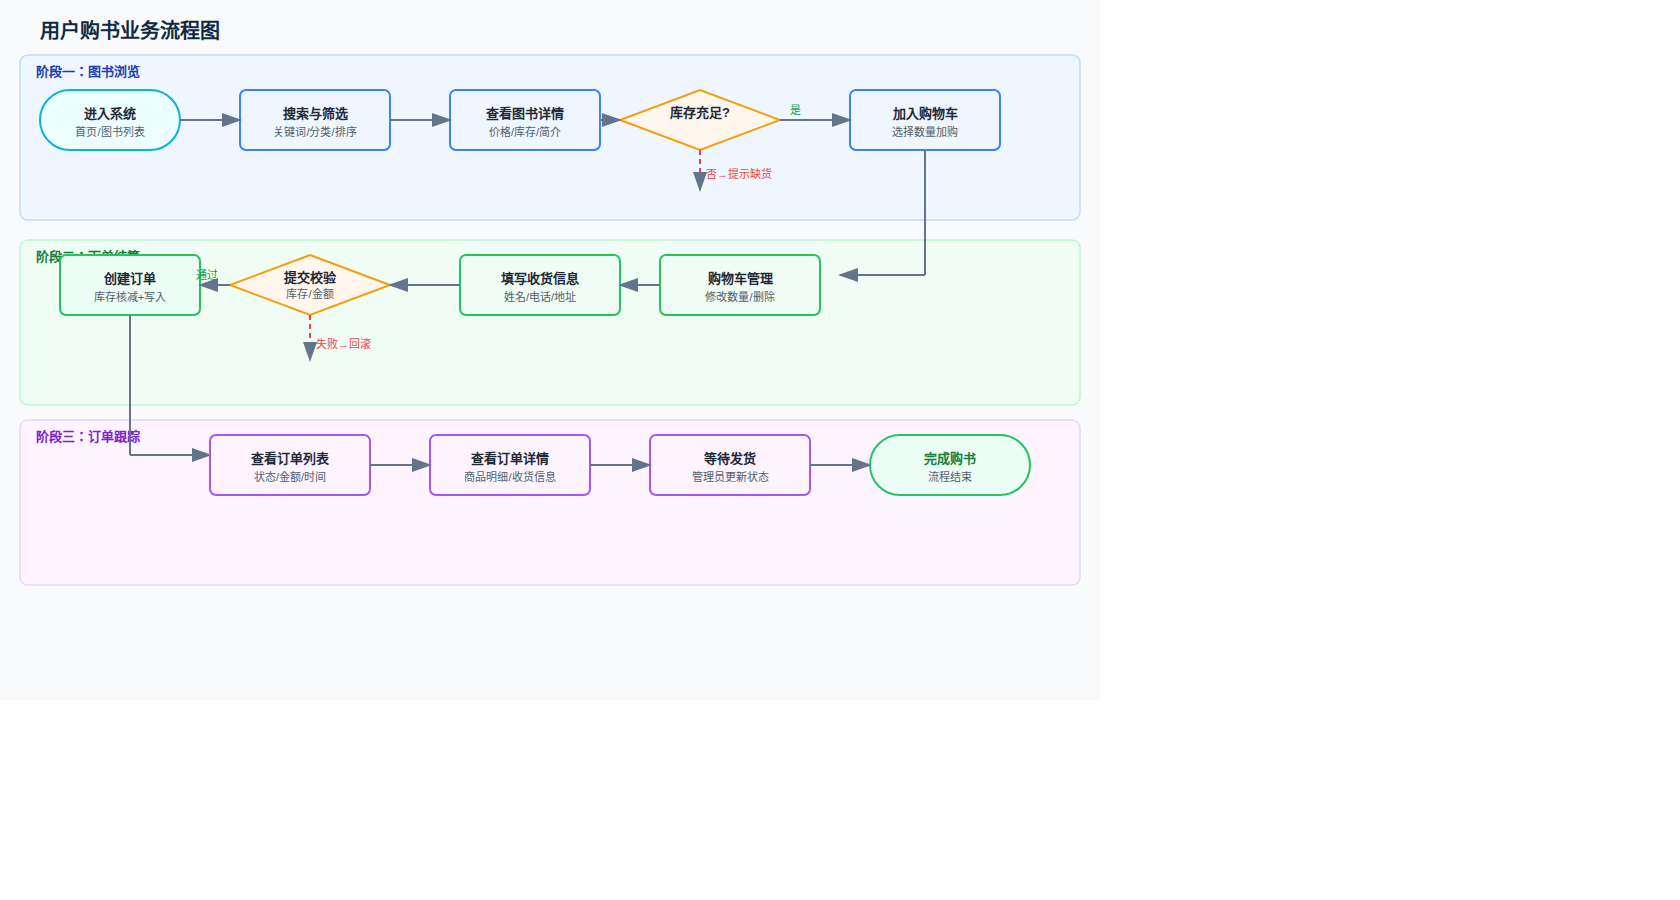
\includegraphics[width=\textwidth]{diagrams/user_purchase_flow.png}
  \caption{用户购书业务流程图}
  \label{fig:user-purchase-flow}
\end{figure}

从该流程可以看出，用户端需求不仅包括页面展示本身，还包括库存校验、订单状态管理和异常场景处理等后台约束。因此，系统在需求设计时必须将页面交互需求与业务规则需求统一考虑，而不能仅停留在静态界面层面。

\subsection{管理员端功能需求分析}

管理员端的目标是保证平台商品数据、分类数据与订单数据的有效运转。与用户端相比，管理员端更加关注数据准确性、状态一致性与操作效率，其功能需求如表\ref{tab:admin-functional-requirements}所示。

\begin{table}[H]
  \centering
  \caption{管理员端功能需求}
  \label{tab:admin-functional-requirements}
  \begin{tabularx}{\textwidth}{p{2.8cm} p{3.2cm} X}
    \toprule
    功能模块 & 子功能 & 需求描述 \\
    \midrule
    后台首页 & 统计信息展示 & 展示订单总量、图书数量、分类数量、用户数量和销售额等关键指标，为管理决策提供依据。 \\
    书籍管理 & 书籍增删改查 & 支持新增图书、编辑图书、删除图书以及上下架状态切换，并允许查看已下架图书。 \\
    分类管理 & 分类增删改查 & 支持新增、编辑与删除图书分类，删除分类时需处理与图书之间的关联关系。 \\
    订单管理 & 订单查询与状态维护 & 支持查看所有订单，并将订单状态从待处理更新为已发货、已完成或已取消。 \\
    经营辅助 & 最近订单与概览信息 & 在管理首页展示最近订单信息，便于在演示和日常使用中快速了解系统运行情况。 \\
    \bottomrule
  \end{tabularx}
\end{table}

后台功能的关键要求不只是“可操作”，还要能够体现完整的 CRUD 闭环，即管理员在新增数据后能够立即查看结果，在编辑后能够验证修改生效，在删除或下架后仍可通过列表状态区分进行管理。该要求对于毕业设计演示尤为重要，因为它直接决定系统能否清晰展示功能完整性。

管理员端的整体职责关系如图\ref{fig:role-module-requirements}和图\ref{fig:admin-crud-flow}所示。

\begin{figure}[H]
  \centering
  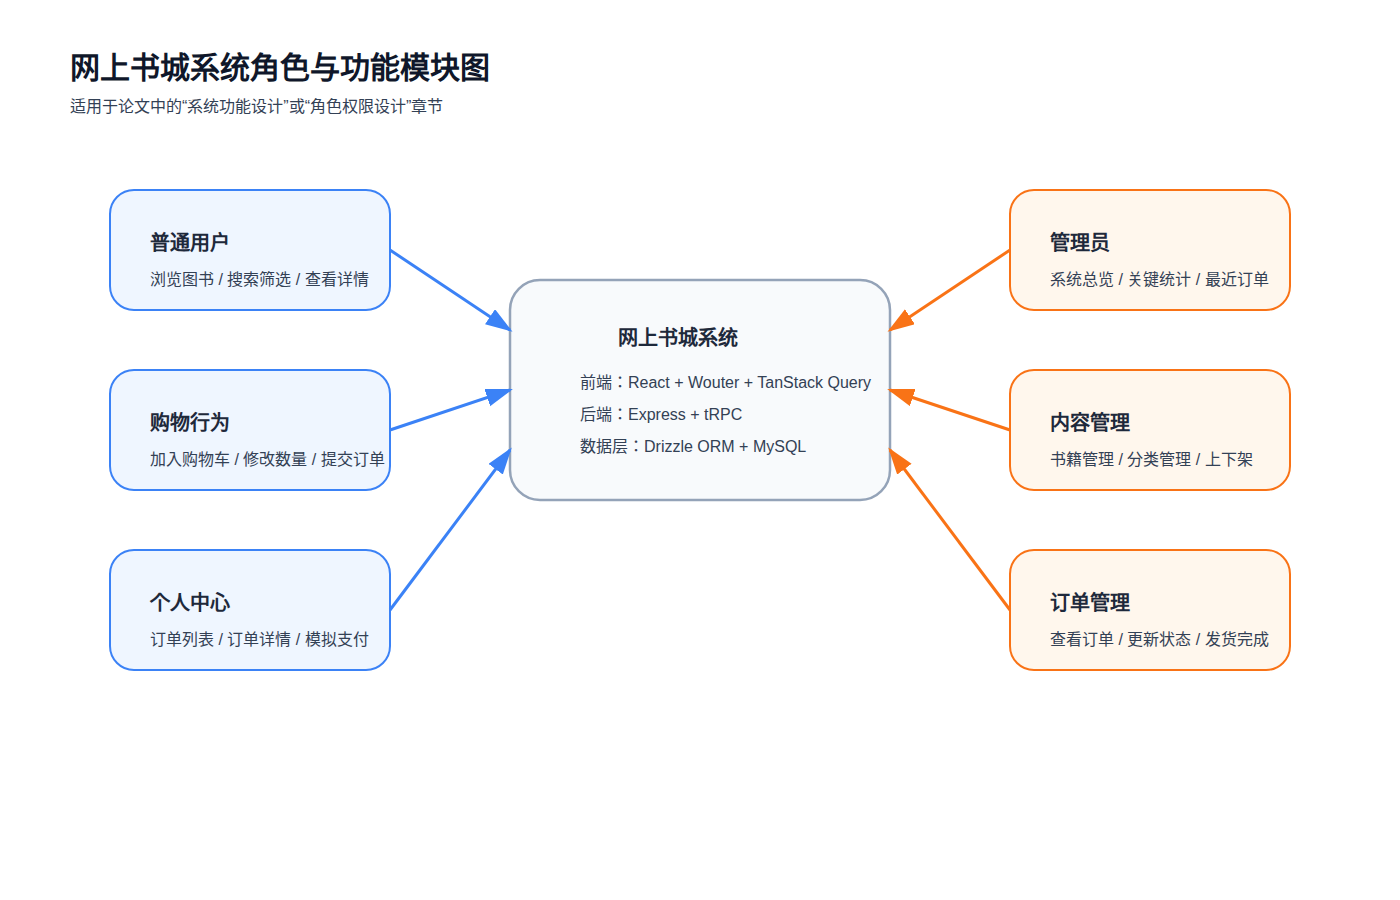
\includegraphics[width=0.95\textwidth]{diagrams/role_module_diagram.png}
  \caption{系统角色与功能模块图}
  \label{fig:role-module-requirements}
\end{figure}

\begin{figure}[H]
  \centering
  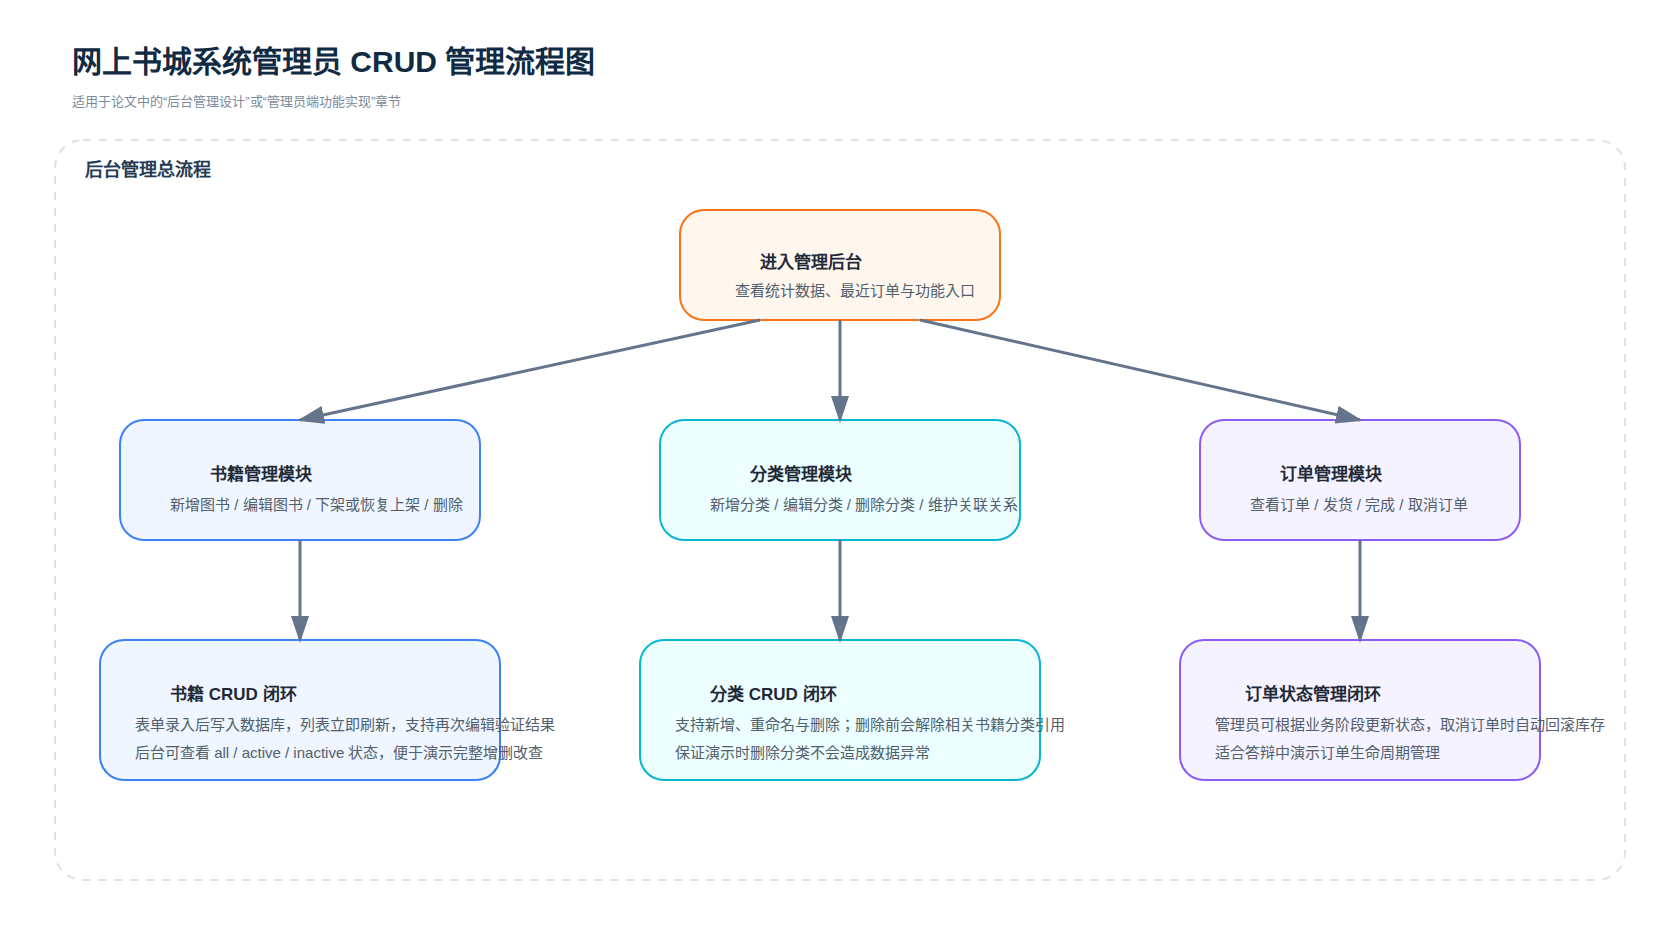
\includegraphics[width=\textwidth]{diagrams/admin_crud_flow.png}
  \caption{管理员 CRUD 管理流程图}
  \label{fig:admin-crud-flow}
\end{figure}

\subsection{业务规则需求分析}

除显性页面功能外，系统还需要满足若干关键业务规则，这些规则决定了系统是否具备真实业务场景下的正确性。

\textbf{库存约束规则。}图书加入购物车与提交订单时均需检查库存是否充足，库存不足时应阻止继续下单，并向用户返回明确提示。若订单被取消，系统还应恢复相应图书库存，以维持数据一致性。

\textbf{图书状态规则。}已下架图书不应继续出现在正常销售流程中，也不允许被新加入购物车或用于订单创建；但管理员应能够在后台查看并恢复该类图书。

\textbf{订单流转规则。}订单状态必须遵循一定的生命周期，例如待支付、待处理、已发货、已完成或已取消。不同状态下允许的操作应受到限制，避免出现已取消订单再次发货或已完成订单被重复取消等异常情况。

\textbf{分类关联规则。}图书与分类之间存在关联关系，当管理员删除分类时，系统应同步处理关联图书的分类字段，防止出现悬空引用或错误数据。

\subsection{非功能需求分析}

除业务功能需求外，系统还需满足一定的非功能需求，以保证其在论文研究与系统演示层面具备较好的完整性和工程价值。

\textbf{易用性需求。}系统界面应保持布局清晰、操作路径明确，用户在不阅读额外说明的前提下即可完成浏览、加购、下单与查询等核心操作。后台页面则应尽量减少跳转层级，将常用管理功能集中展示。

\textbf{性能需求。}在常规校园网络环境下，首页、图书列表页与后台首页应能够在较短时间内完成加载。对于常见查询操作，系统应保证响应延迟处于可接受范围，以避免频繁等待影响演示效果。

设接口平均响应时间为$T_{\text{avg}}$，系统设计目标可表示为：
\begin{equation}
  T_{\text{avg}} \leq 200\text{ ms},\quad T_{\text{p95}} \leq 500\text{ ms}
  \label{eq:perf-target}
\end{equation}

\textbf{安全性需求。}系统需具备基本身份鉴别与权限控制能力。普通用户敏感操作要求登录后进行，管理员接口必须进行角色校验；密码等敏感数据需使用哈希方式存储，避免明文保存。

\textbf{可维护性需求。}由于本系统采用 React、tRPC 与 Drizzle ORM 的全栈 TypeScript 技术路线，因此需要保证数据类型定义在前后端之间保持一致，减少传统接口文档与实体定义重复维护带来的负担。

\textbf{可演示性需求。}作为毕业设计系统，平台不仅要在代码层面可运行，还要在界面层面能够完整展示用户端与管理员端的核心流程。因此，系统需要具备较完整的样例数据、明确的空状态提示以及稳定的关键页面展示效果。

\subsection{本章小结}

本章从系统角色、用户端功能、管理员端功能、业务规则以及非功能性约束五个方面对网上书城系统进行了需求分析。通过分析可以看出，系统不仅需要完成图书销售的基本业务流程，还要兼顾后台 CRUD 管理闭环、库存与订单状态一致性以及前后端协作效率等工程要求。这些需求为后续的系统架构设计、数据库建模和模块实现提供了明确依据。

% ======== 第3章 系统设计 ========
\section{系统设计}

\subsection{整体架构设计}

系统采用前后端分离的整体架构。前端以React 18构建单页应用，由Vite负责开发服务与生产构建；后端基于Node.js与Express提供HTTP服务，tRPC框架在其上封装类型安全的远程过程调用层；持久层由Drizzle ORM操作MySQL数据库，Schema定义文件同时承担数据迁移与类型推导两项职责。三层之间的依赖关系单向流动，不存在跨层的直接引用。

与传统REST方案相比，tRPC的核心差异在于接口协议的定义位置。设服务端过程定义为$P$，其输入类型为$I$，输出类型为$O$，则前端调用层自动获得类型约束：
\begin{equation}
  \text{client}(P) : I \rightarrow \text{Promise}\langle O \rangle
  \label{eq:trpc-type}
\end{equation}

这一机制消除了手工维护接口文档的必要性，接口字段的重命名或类型变更能够立即在前端调用处产生编译错误，而非在运行时以网络请求失败的形式暴露。

系统总体架构如图\ref{fig:system-architecture}所示。普通用户端与管理员端通过浏览器访问同一前端单页应用，前端借助tRPC Client将类型安全的请求发送到Express服务端；服务端在完成会话校验、权限判断与业务处理后，通过Drizzle ORM访问MySQL数据库，从而形成较清晰的四层协作结构。

\begin{figure}[H]
  \centering
  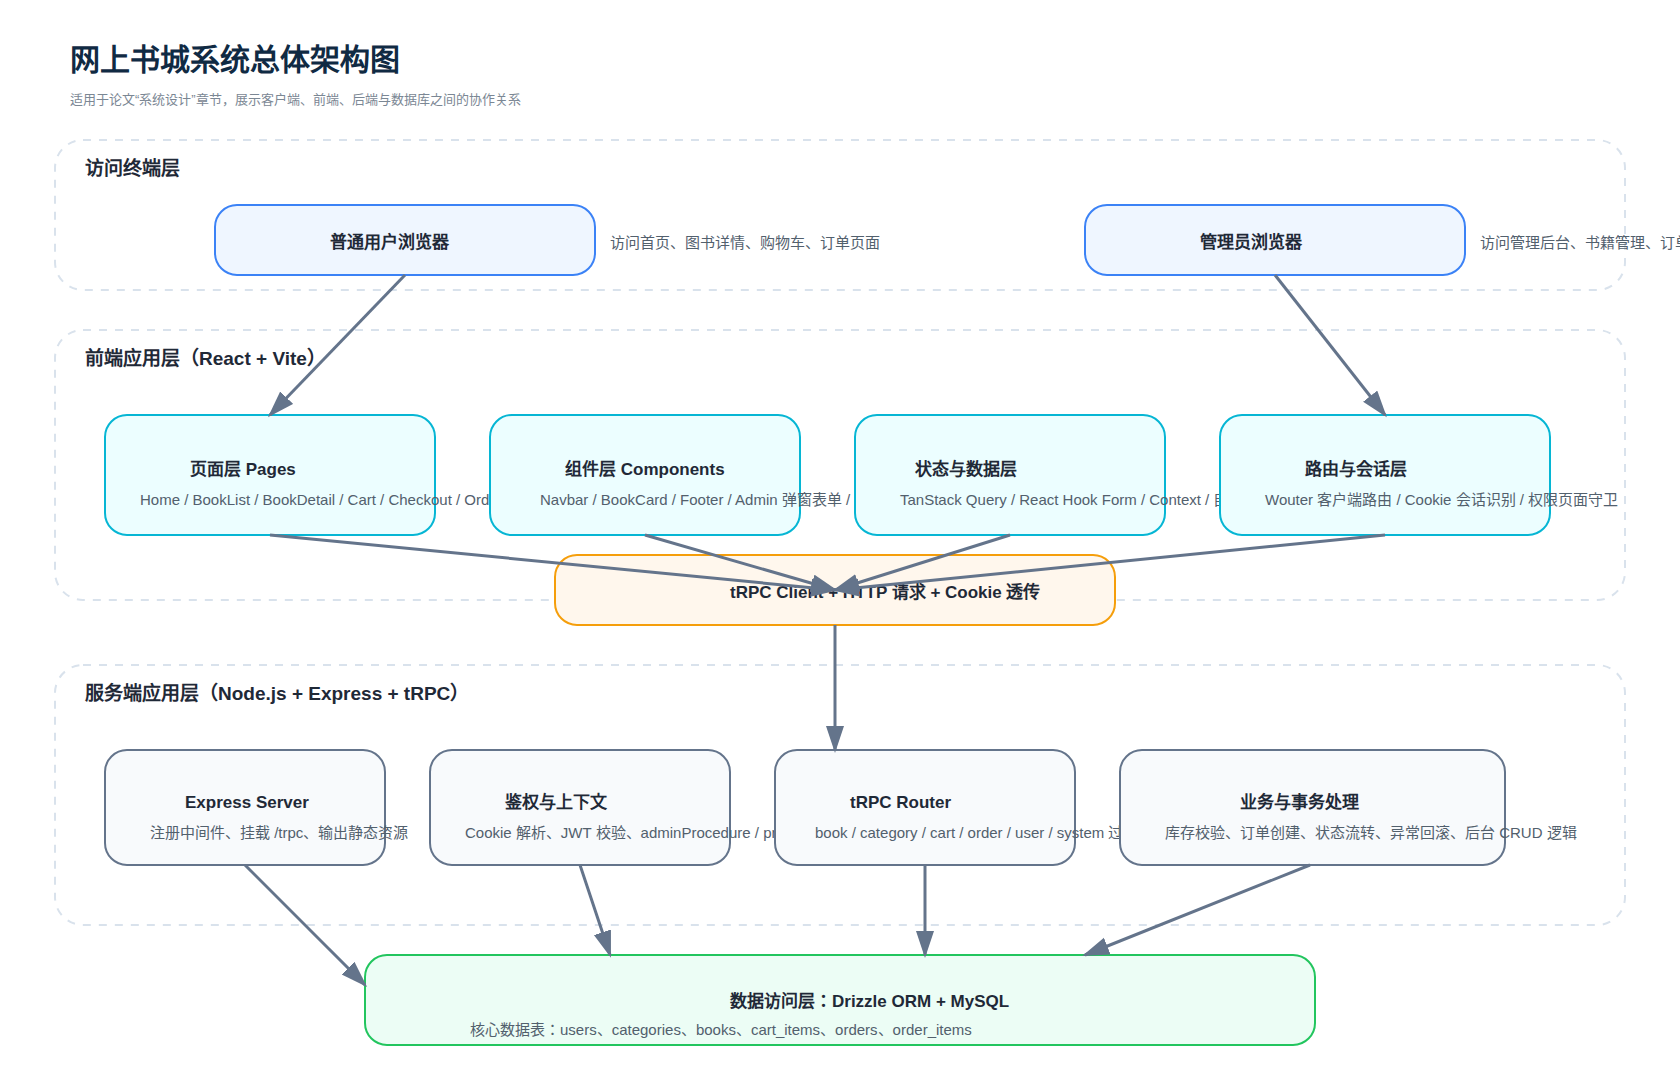
\includegraphics[trim=24 20 24 16, clip, width=\textwidth]{diagrams/system_architecture_diagram.png}
  \caption{系统总体架构图}
  \label{fig:system-architecture}
\end{figure}

\subsection{前端架构设计}

前端目录结构遵循关注点分离原则：\texttt{pages/}存放页面级组件，负责数据获取与布局编排；\texttt{components/}存放可复用的业务组件；\texttt{components/ui/}存放基于shadcn/ui封装的原子级UI组件；\texttt{hooks/}存放与具体页面解耦的业务逻辑Hook；\texttt{contexts/}存放跨组件共享的上下文状态。

数据请求层由TanStack Query统一管理，tRPC客户端以React Query适配器的形式注入，页面组件通过\texttt{trpc.xxx.useQuery()}与\texttt{trpc.xxx.useMutation()}发起请求，请求状态由框架自动维护，组件无需手动管理\texttt{loading}状态变量。路由采用wouter库实现客户端路由，体积轻量且API风格与React Router基本一致。

\subsection{后端架构设计}

服务端入口文件注册Express中间件链，依次处理CORS跨域、Cookie解析、JSON请求体解析，最后将\texttt{/trpc}路径下的所有请求转发至tRPC适配器。tRPC Router按功能域拆分为\texttt{bookRouter}、\texttt{categoryRouter}、\texttt{orderRouter}、\texttt{userRouter}四个子路由，合并后挂载至根Router。

权限控制通过tRPC中间件实现。公开接口使用公开过程；需要登录的接口使用受保护过程；管理员接口使用管理员过程。三类过程通过中间件链式组合完成上下文增强与权限收敛，鉴权逻辑集中在中间件层，业务过程函数无需重复处理权限细节。

\subsection{数据库设计}

数据库采用MySQL，共设计六张核心数据表，以Drizzle ORM的TypeScript Schema定义为唯一数据源，表结构说明如表\ref{tab:db-tables}所示。

\begin{table}[H]
  \centering
  \caption{数据库核心表结构说明}
  \label{tab:db-tables}
  \begin{tabularx}{\textwidth}{p{2.5cm} p{5.1cm} X}
    \toprule
    表名 & 主要字段 & 说明 \\
    \midrule
    users & id, openId, name, email, role & 用户基本信息，role枚举区分普通用户与管理员 \\
    categories & id, name, description & 图书分类，name字段设唯一约束 \\
    books & id, title, author, price, stock, salesCount, categoryId & 图书主表，price精度(10,2)，外键关联categories \\
    cart\_items & id, userId, bookId, quantity & 购物车明细，避免同一用户重复加购同一书籍 \\
    orders & id, userId, totalAmount, status, shippingAddress & 订单主表，status枚举覆盖完整状态流转 \\
    order\_items & id, orderId, bookId, quantity, price & 订单明细，price记录下单时价格快照 \\
    \bottomrule
  \end{tabularx}
\end{table}

订单明细表在写入时保存当时的书籍单价快照，确保历史订单金额不受后续调价影响，这是电商系统处理价格一致性的常见设计范式。设某订单含$n$个品种，第$i$种书籍数量为$q_i$，下单时单价为$p_i$，则订单总金额满足：
\begin{equation}
  M = \sum_{i=1}^{n} q_i \cdot p_i
  \label{eq:order-total}
\end{equation}

各核心数据表之间的关系如图\ref{fig:database-er}所示。该设计以\texttt{users}表作为用户主体，以\texttt{books}和\texttt{categories}构成商品主数据，以\texttt{cart\_items}、\texttt{orders}和\texttt{order\_items}共同描述用户从加购到下单的业务链路。

\begin{figure}[H]
  \centering
  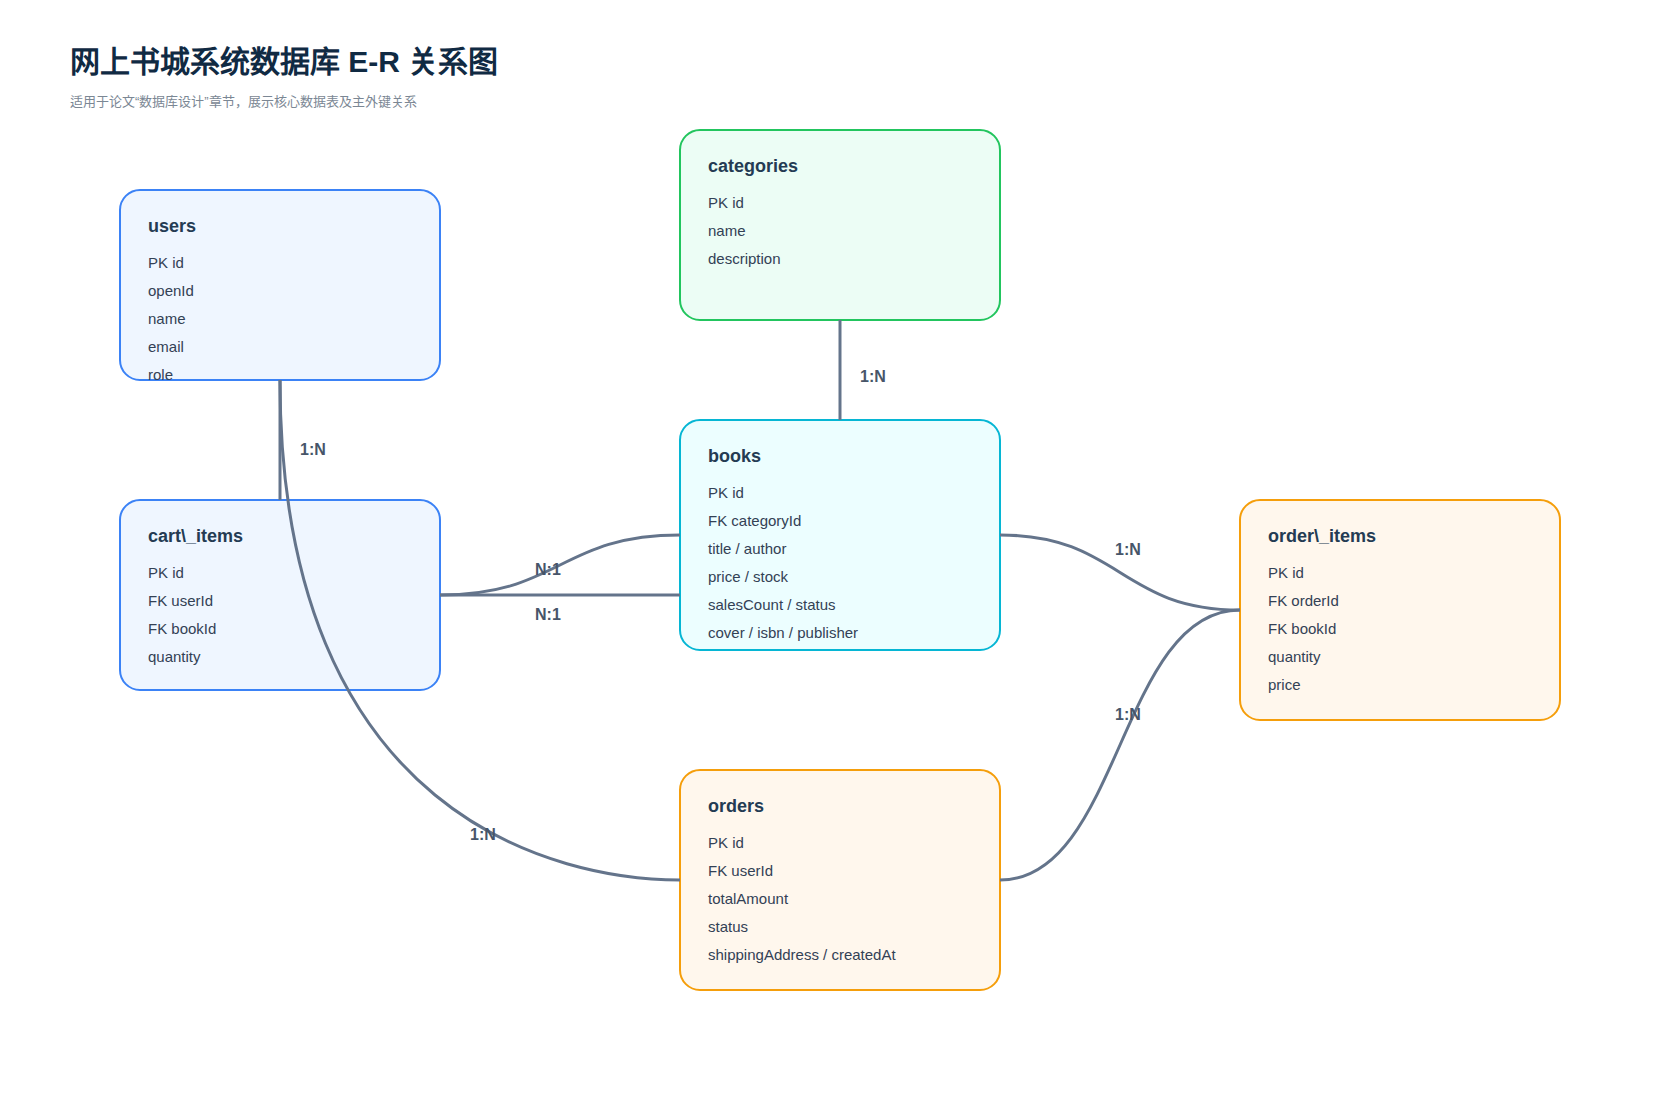
\includegraphics[trim=22 18 22 16, clip, width=\textwidth]{diagrams/database_er_diagram.png}
  \caption{数据库 E-R 关系图}
  \label{fig:database-er}
\end{figure}

\subsection{系统页面结构与业务流程}

系统前端共包含十个路由页面，用户端与管理员端共用同一React应用入口。页面间导航关系如图\ref{fig:ui-structure}所示，首页作为流量入口分发至图书列表、分类检索等子流程，购物车与订单模块通过顶部导航栏全局可达。

\begin{figure}[H]
  \centering
  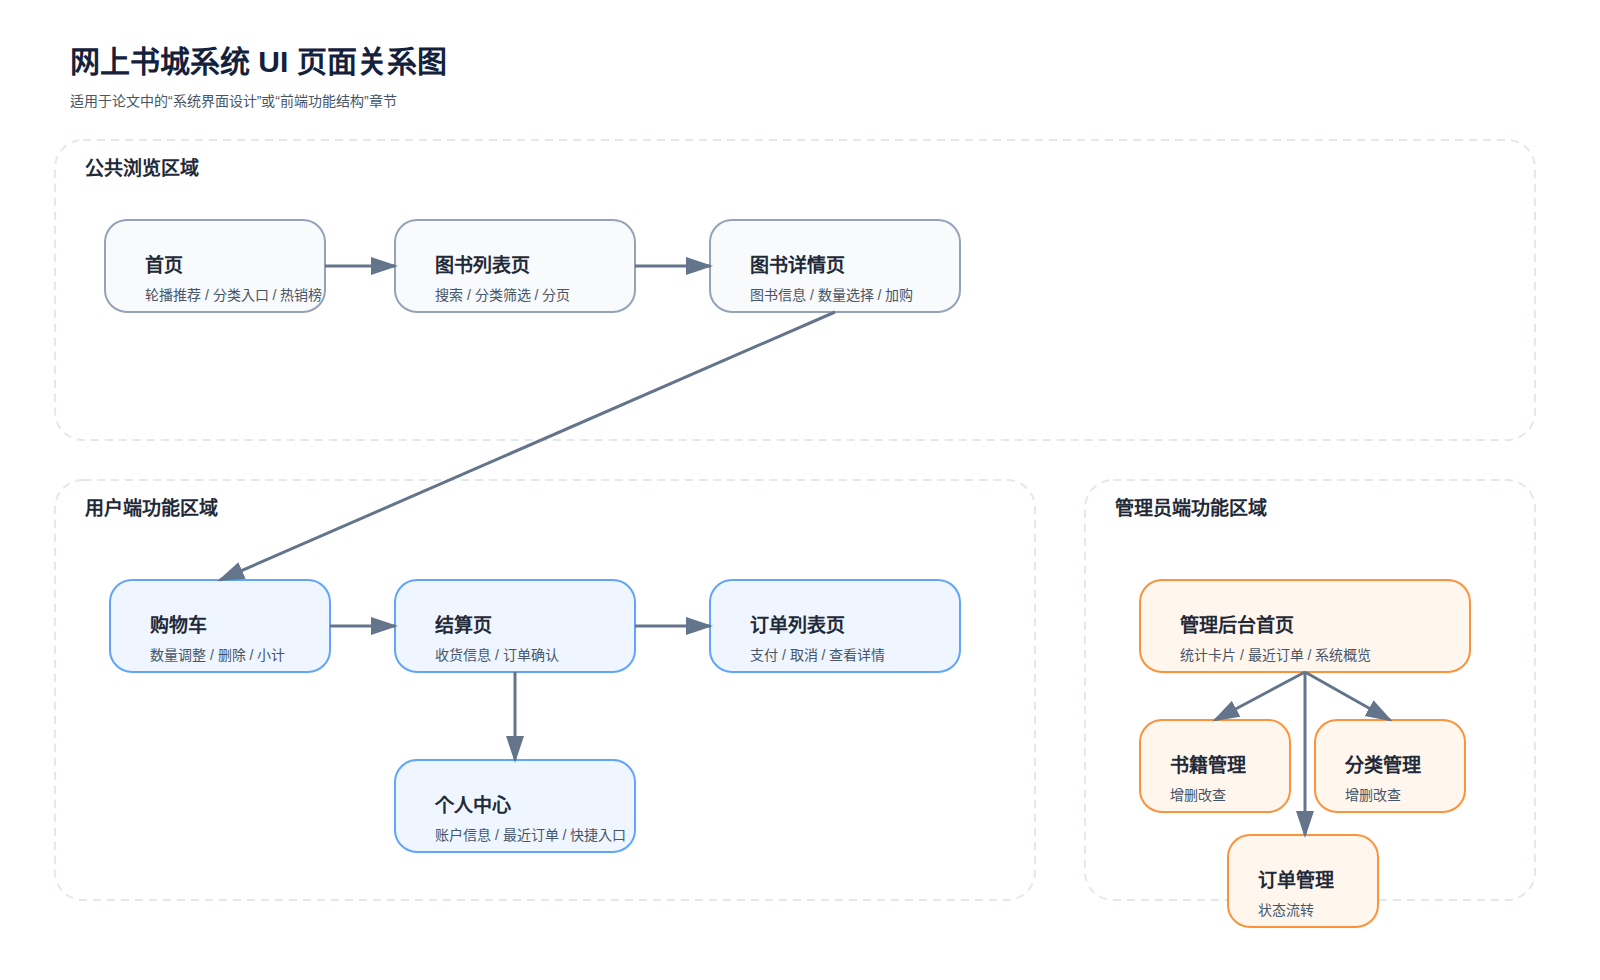
\includegraphics[trim=24 20 24 18, clip, width=\textwidth]{diagrams/ui_page_structure.png}
  \caption{系统UI页面关系图}
  \label{fig:ui-structure}
\end{figure}

系统角色与功能模块的对应关系如图\ref{fig:role-module}所示，普通用户与管理员功能边界严格隔离，管理员端模块均须经过服务端权限校验方可访问。

\begin{figure}[H]
  \centering
  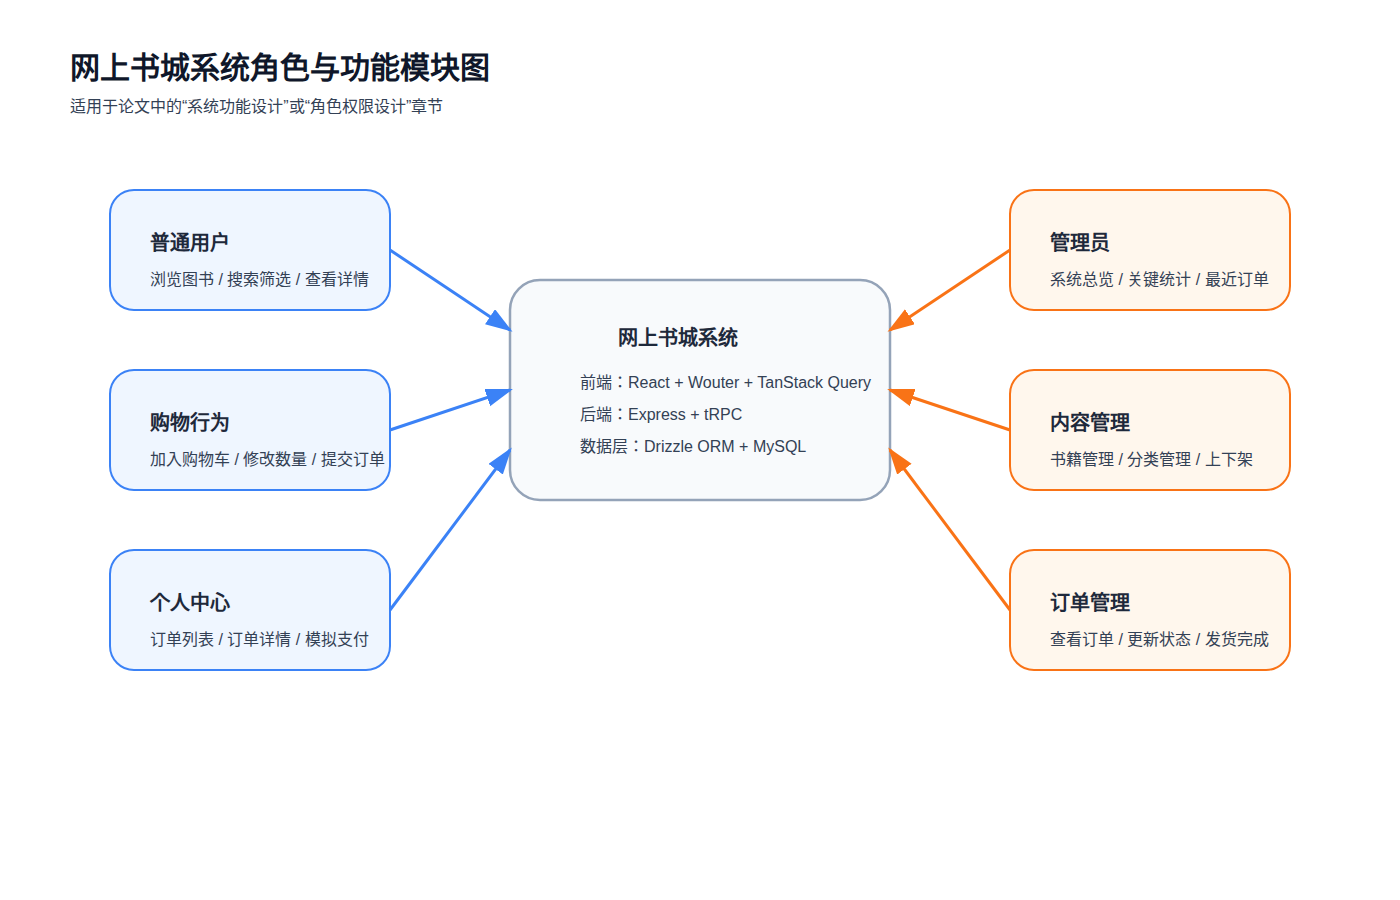
\includegraphics[trim=20 16 20 14, clip, width=0.96\textwidth]{diagrams/role_module_diagram.png}
  \caption{系统角色与功能模块图}
  \label{fig:role-module}
\end{figure}

用户完成一次购书的完整业务流程如图\ref{fig:purchase-flow}所示。用户在详情页选定数量后触发加购，服务端校验库存充足后将明细写入\texttt{cart\_items}表；用户在购物车页填写收货信息后提交订单，服务端在单个数据库事务内完成库存核减与订单记录创建，任一步骤失败均回滚，保证数据一致性。

\begin{figure}[H]
  \centering
  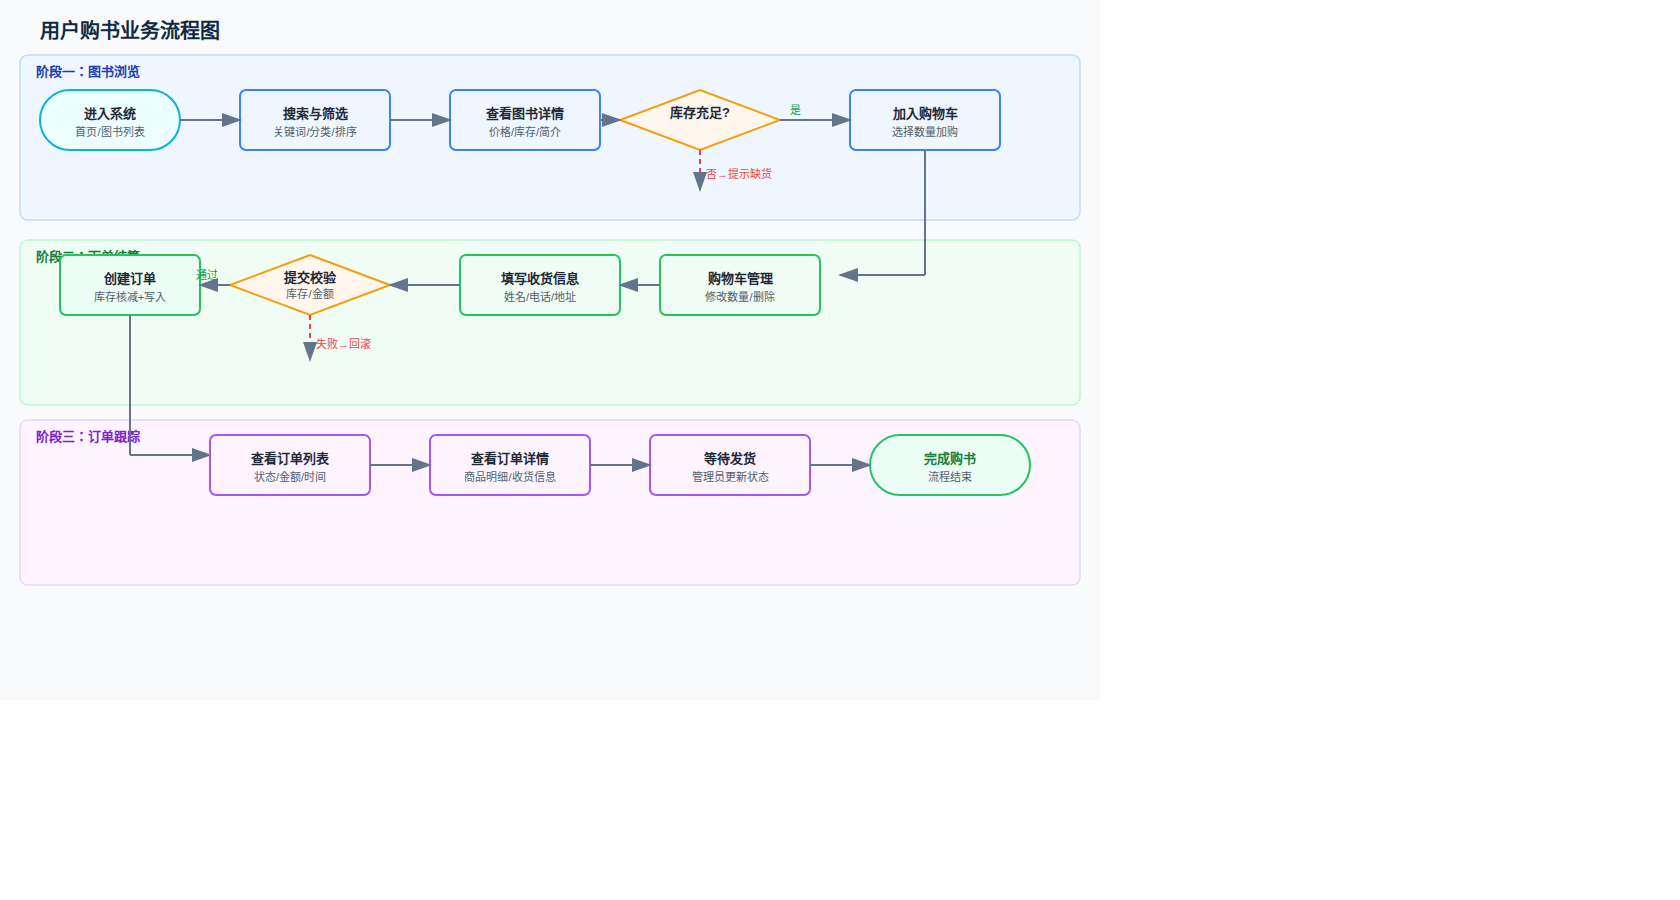
\includegraphics[trim=24 18 24 16, clip, width=\textwidth]{diagrams/user_purchase_flow.png}
  \caption{用户购书业务流程图}
  \label{fig:purchase-flow}
\end{figure}

管理员端的CRUD操作流程如图\ref{fig:admin-flow}所示，书籍与分类管理采用统一的增删改查闭环，订单管理在此基础上增加了状态流转的单向约束：订单状态只允许正向推进，不支持回退至前序状态，以保证业务语义的完整性。

\begin{figure}[H]
  \centering
  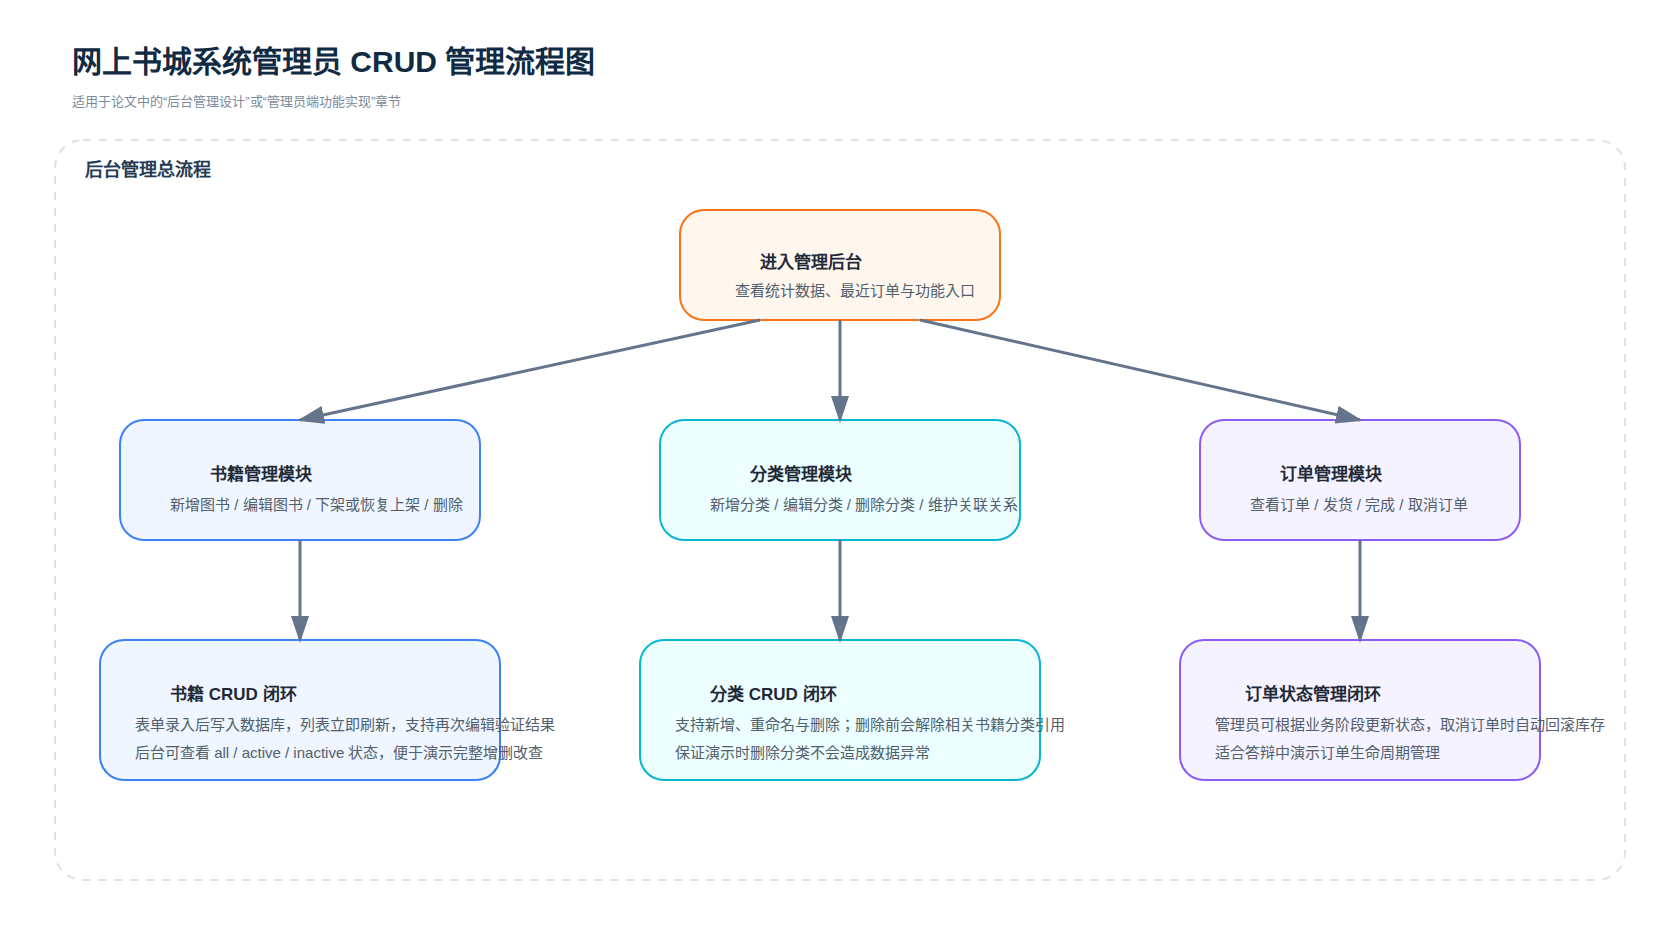
\includegraphics[trim=24 18 24 16, clip, width=\textwidth]{diagrams/admin_crud_flow.png}
  \caption{管理员CRUD管理流程图}
  \label{fig:admin-flow}
\end{figure}

\subsection{本章小结}

本章围绕整体架构、前端设计、后端设计、数据库设计以及系统页面与业务流程五个方面完成了系统设计描述。通过统一的技术选型与分层结构，系统在功能闭环、权限控制、数据一致性与前后端协作效率之间取得了较好的平衡，为后续实现章节提供了结构化依据。


% ======== 第4章 系统实现 ========
\section{系统实现}

\subsection{用户端界面实现}

\subsubsection{首页}

首页由Hero横幅区、服务特性栏、图书分类区与热销/新书推荐区四部分组成。分类数据通过\texttt{trpc.category.list.useQuery()}拉取，热销区与新书区分别以不同\texttt{sortBy}参数复用同一接口，TanStack Query对两次请求独立缓存。如图\ref{fig:home}所示，首页整体风格简洁，BookCard组件在热销区与图书列表页统一复用，保持视觉语言一致。

\begin{figure}[H]
  \centering
  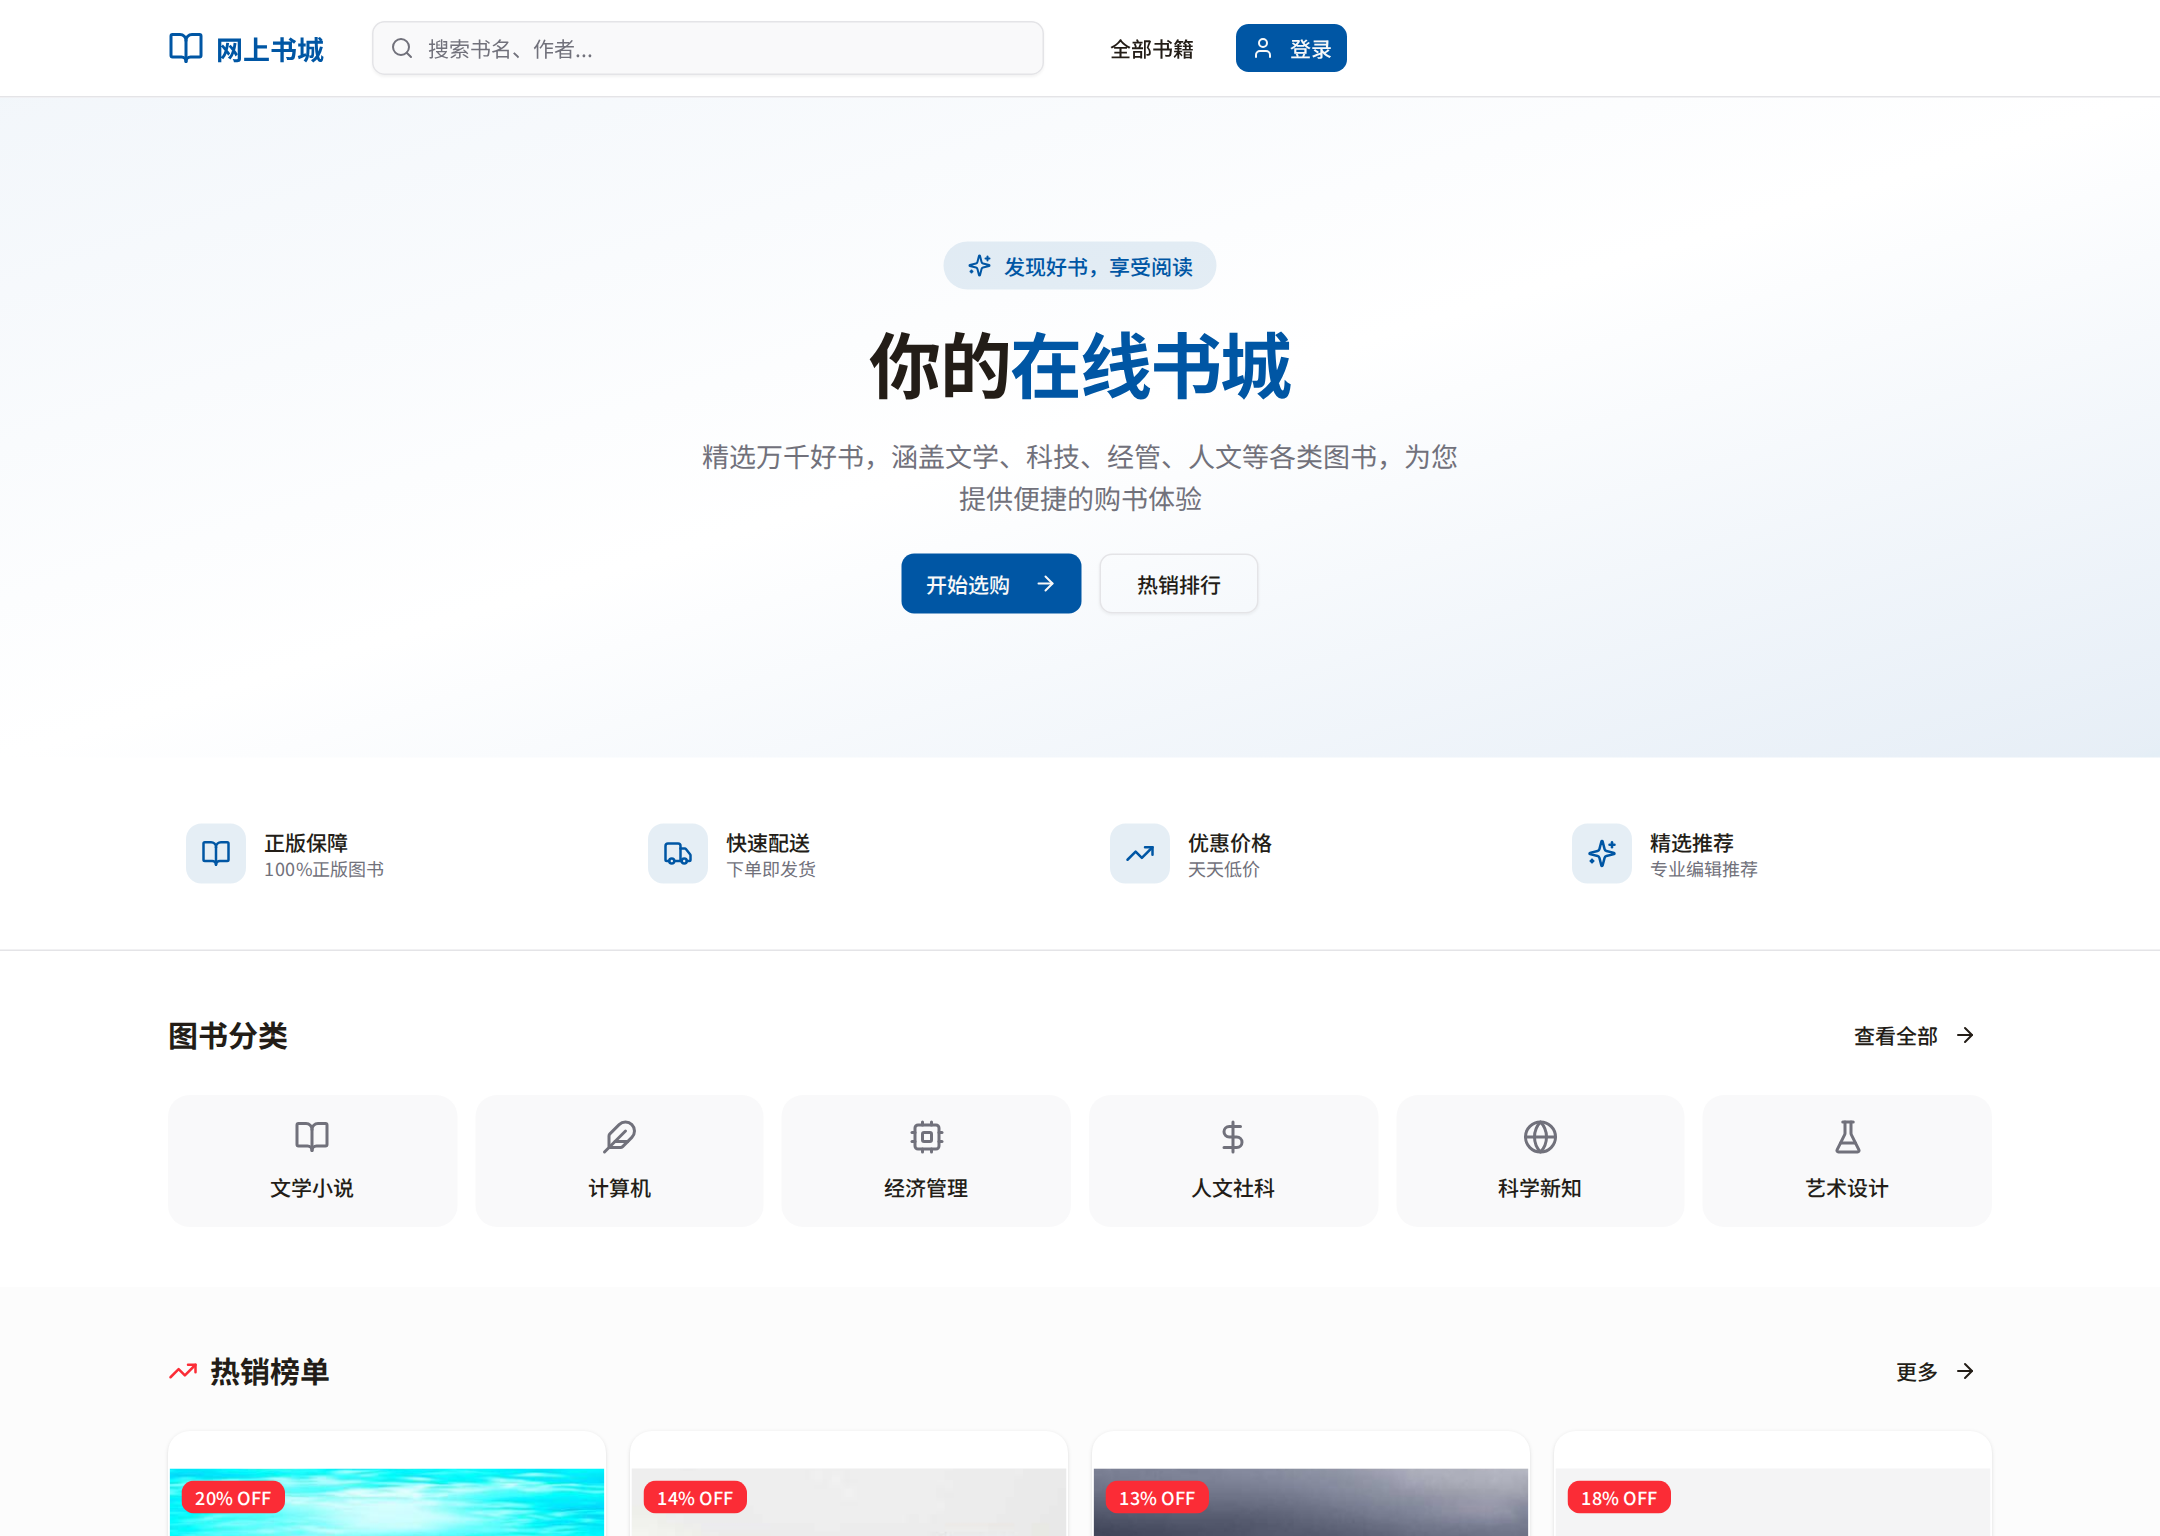
\includegraphics[width=0.90\textwidth]{screenshots/01-home.png}
  \caption{系统首页界面}
  \label{fig:home}
\end{figure}

\subsubsection{图书列表与检索}

图书列表页支持关键词搜索、分类筛选与多维排序，筛选状态通过URL查询参数持久化，刷新或分享链接后状态不丢失。每次筛选条件变更后页码自动重置为第1页，防止越界请求。列表区域采用响应式网格布局，宽屏每行展示四本书，窄屏自动收缩为两列。

\begin{figure}[H]
  \centering
  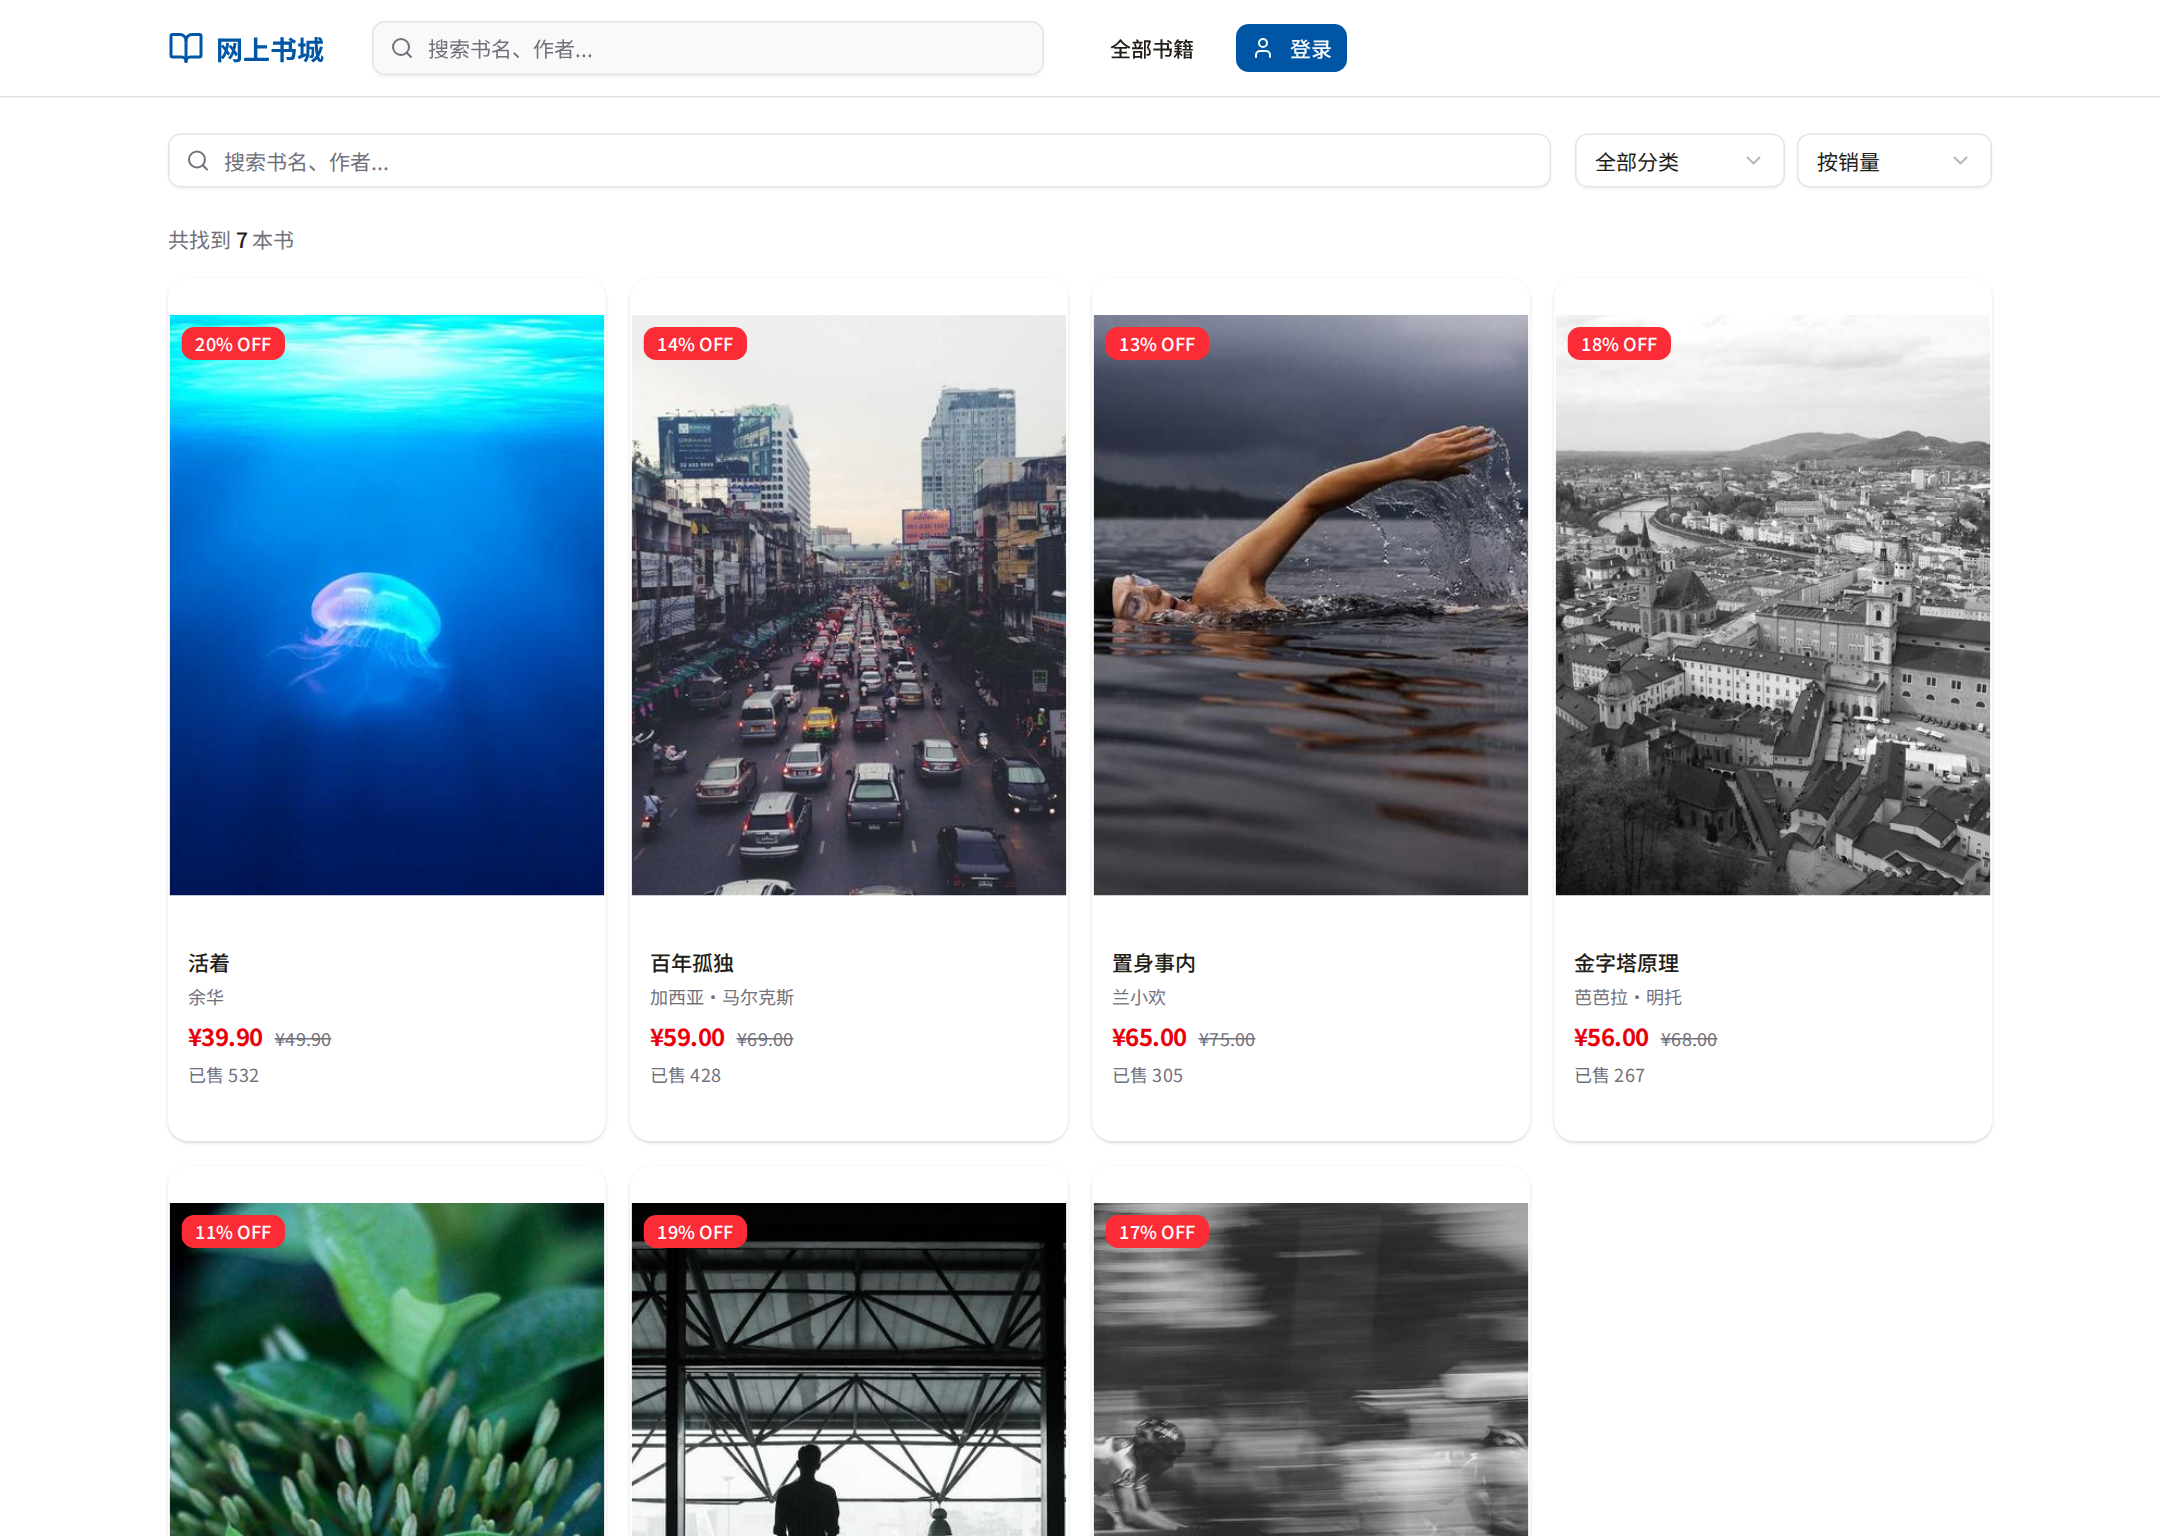
\includegraphics[width=0.90\textwidth]{screenshots/02-book-list.png}
  \caption{图书列表与检索界面}
  \label{fig:booklist}
\end{figure}

\subsubsection{图书详情}

图书详情页展示封面大图、书名、作者、出版社、ISBN、价格、库存及简介。用户选择数量后点击加入购物车，前端即时校验数量不超过当前库存，服务端在写入前再次验证，形成双重防护。

\begin{figure}[H]
  \centering
  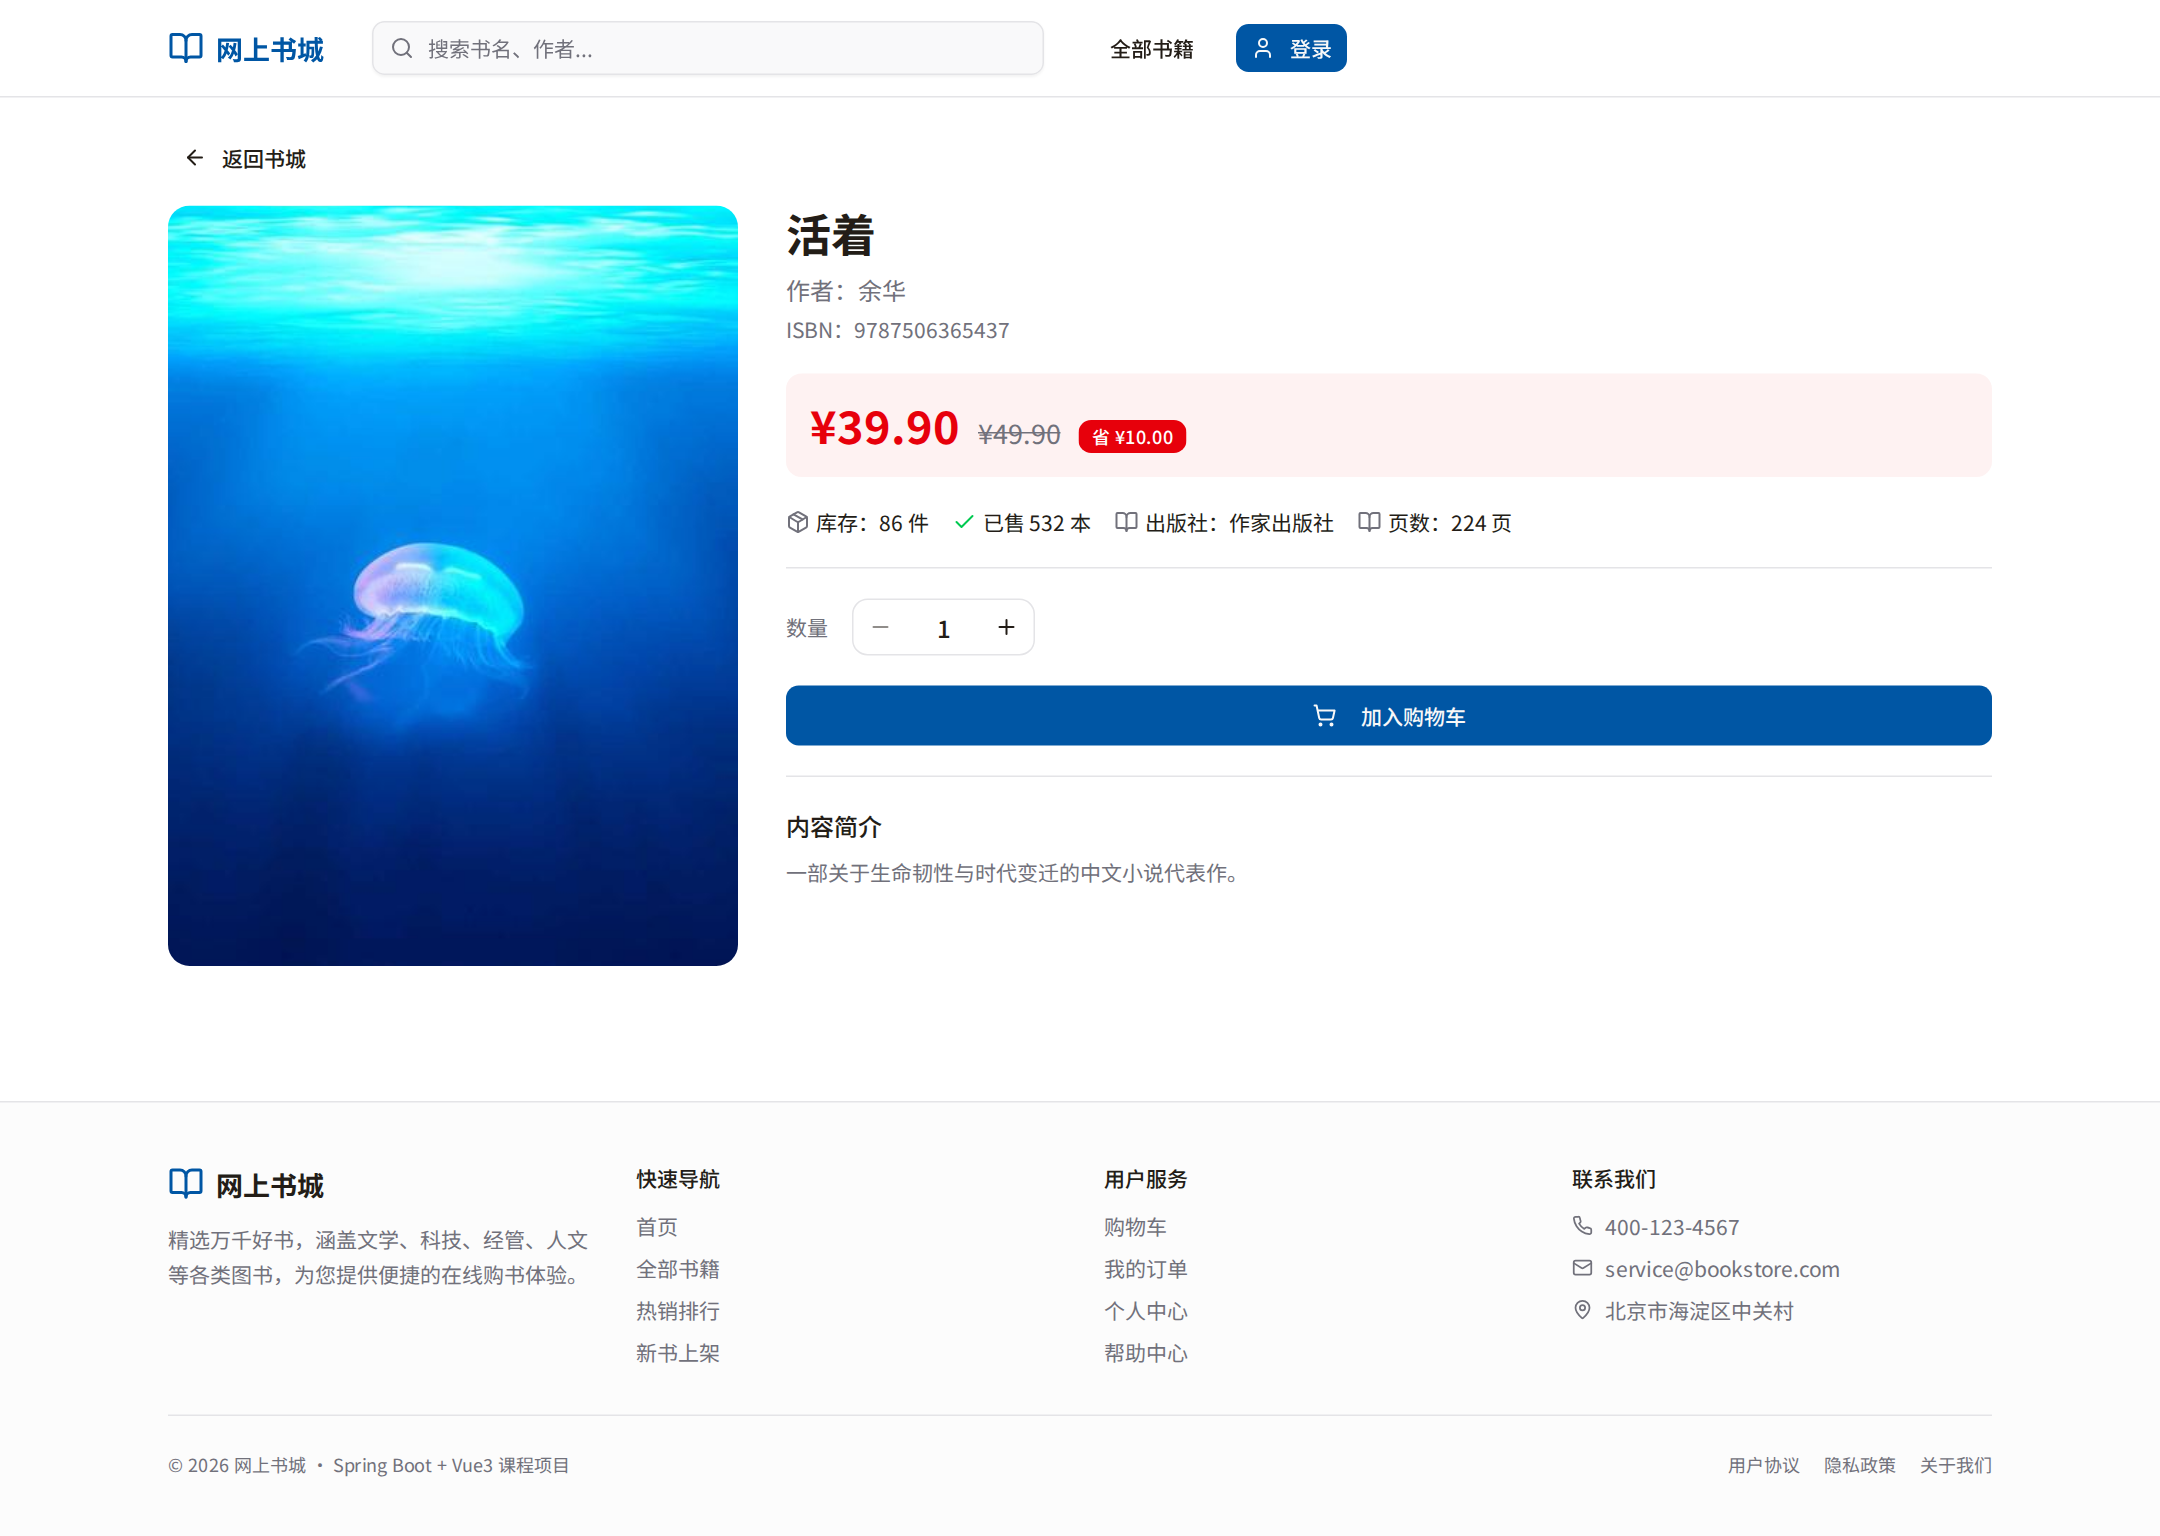
\includegraphics[width=0.90\textwidth]{screenshots/03-book-detail.png}
  \caption{图书详情界面}
  \label{fig:bookdetail}
\end{figure}

\subsubsection{购物车与结算}

购物车页面展示已加购书目，支持数量增减与删除，底部实时汇总金额（依据公式\eqref{eq:order-total}计算）。结算页由react-hook-form与zod schema共同完成表单校验，类型约束与校验规则在同一处定义。提交后服务端在数据库事务中完成库存核减与订单写入，任一步骤失败均回滚。

\begin{figure}[H]
  \centering
  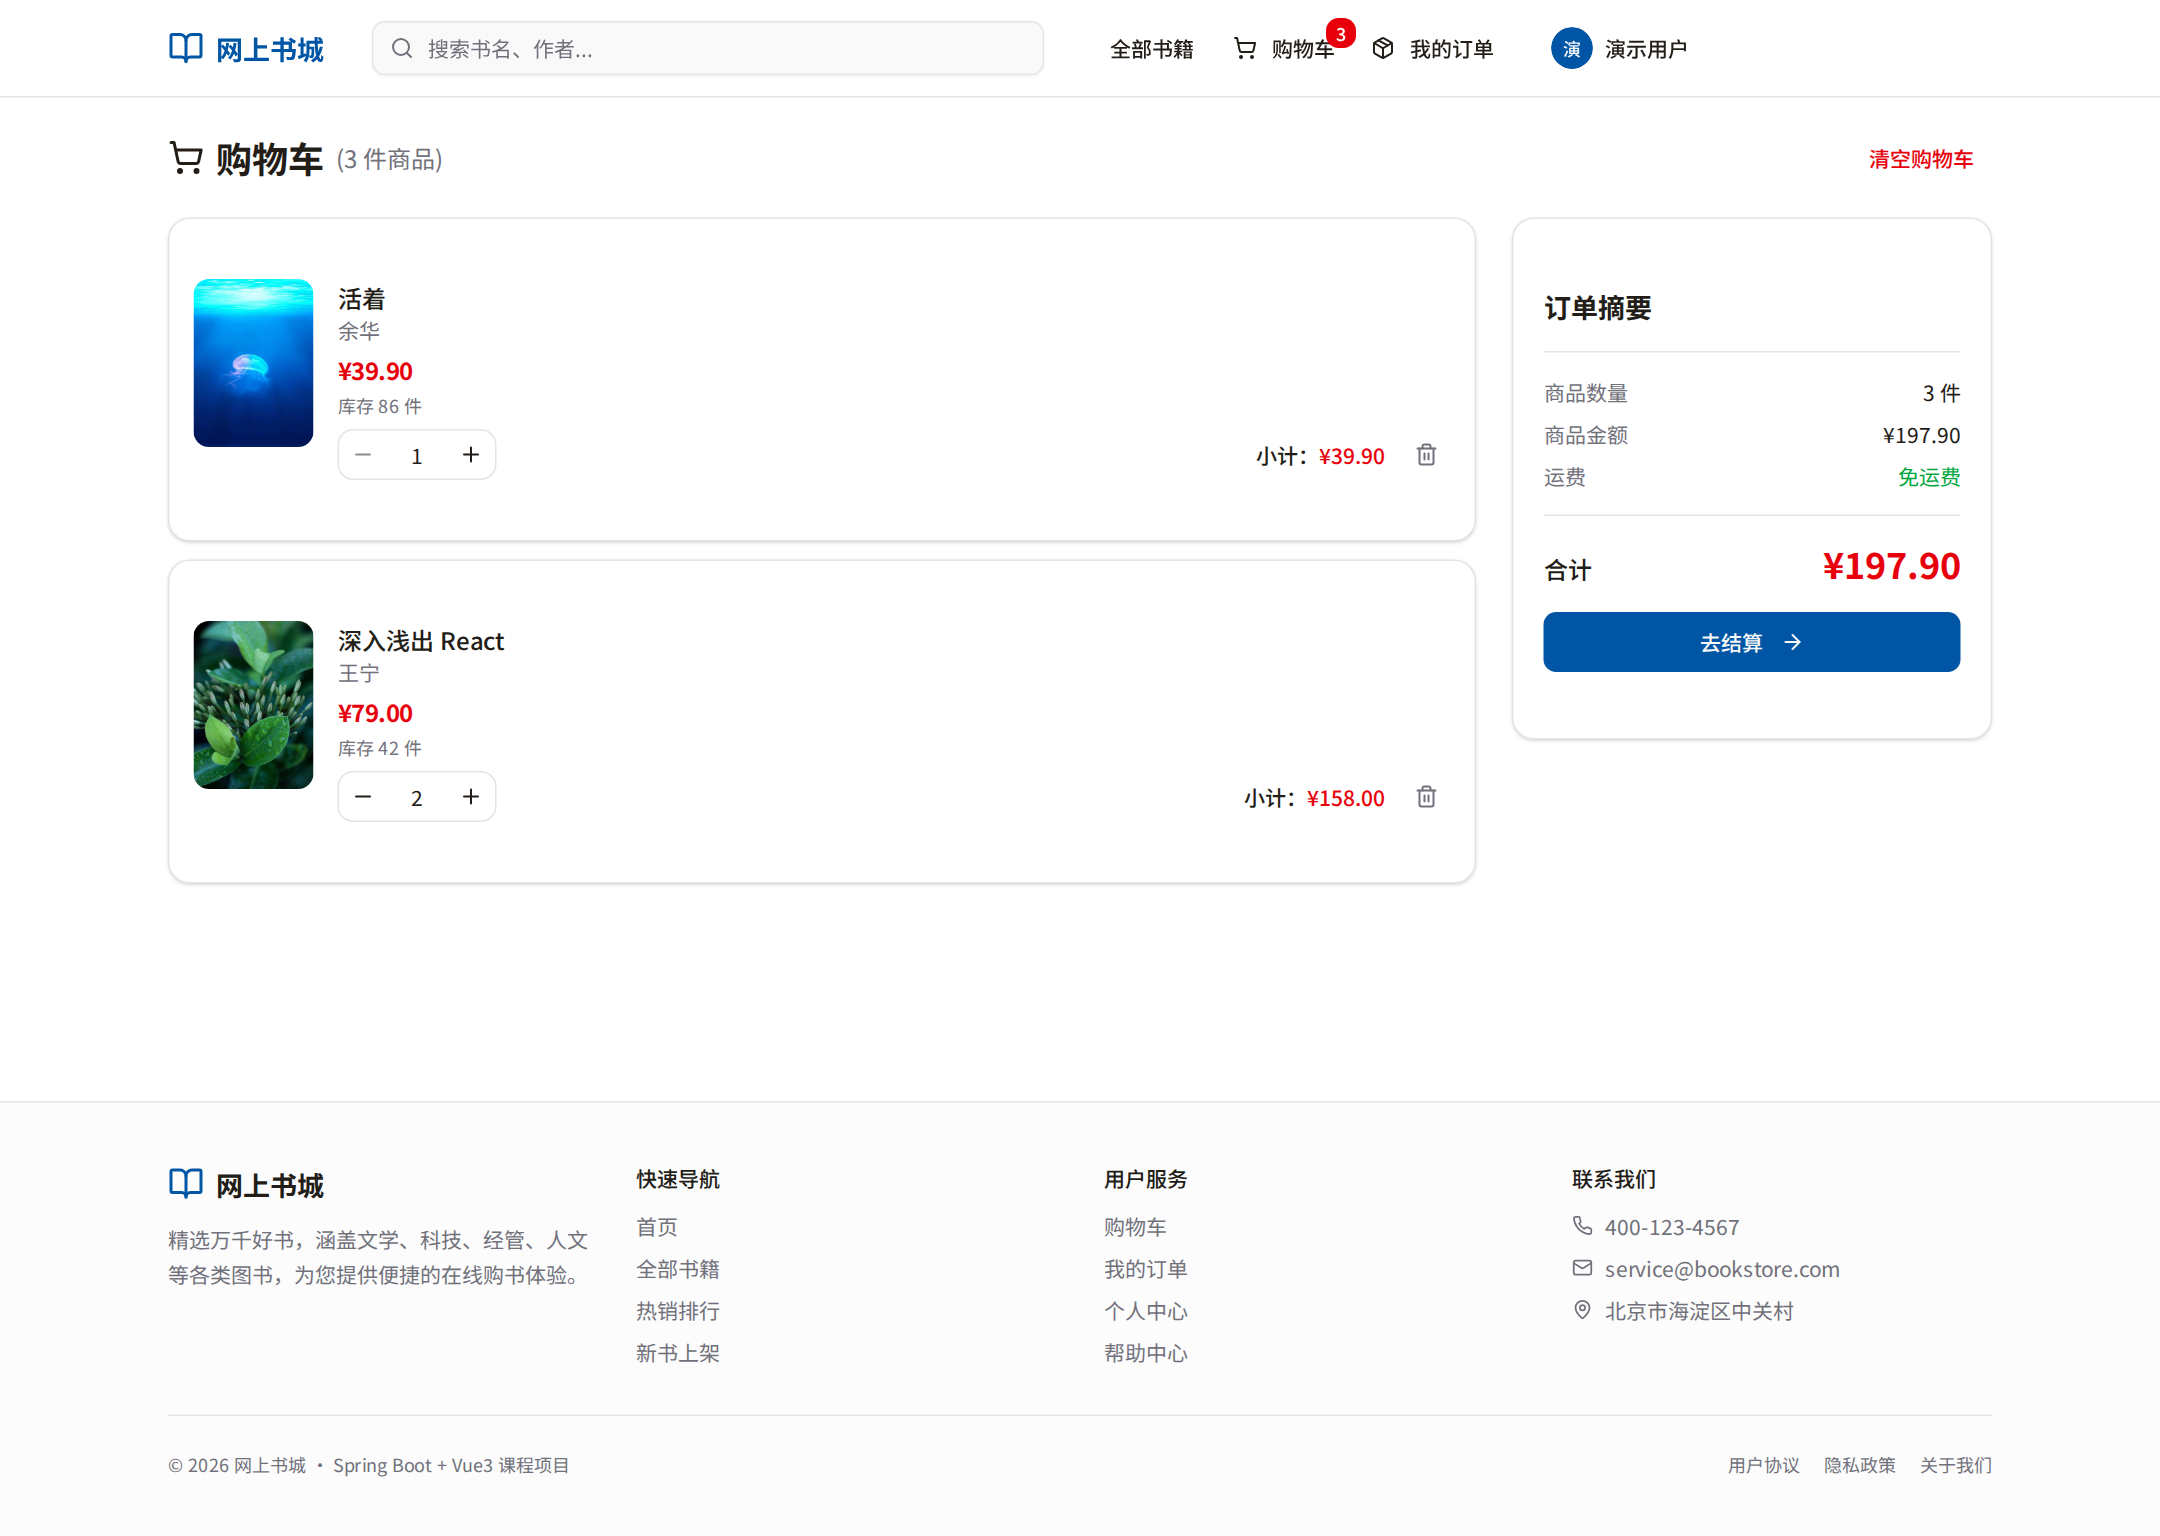
\includegraphics[width=0.90\textwidth]{screenshots/04-user-cart.png}
  \caption{购物车管理界面}
  \label{fig:cart}
\end{figure}

\begin{figure}[H]
  \centering
  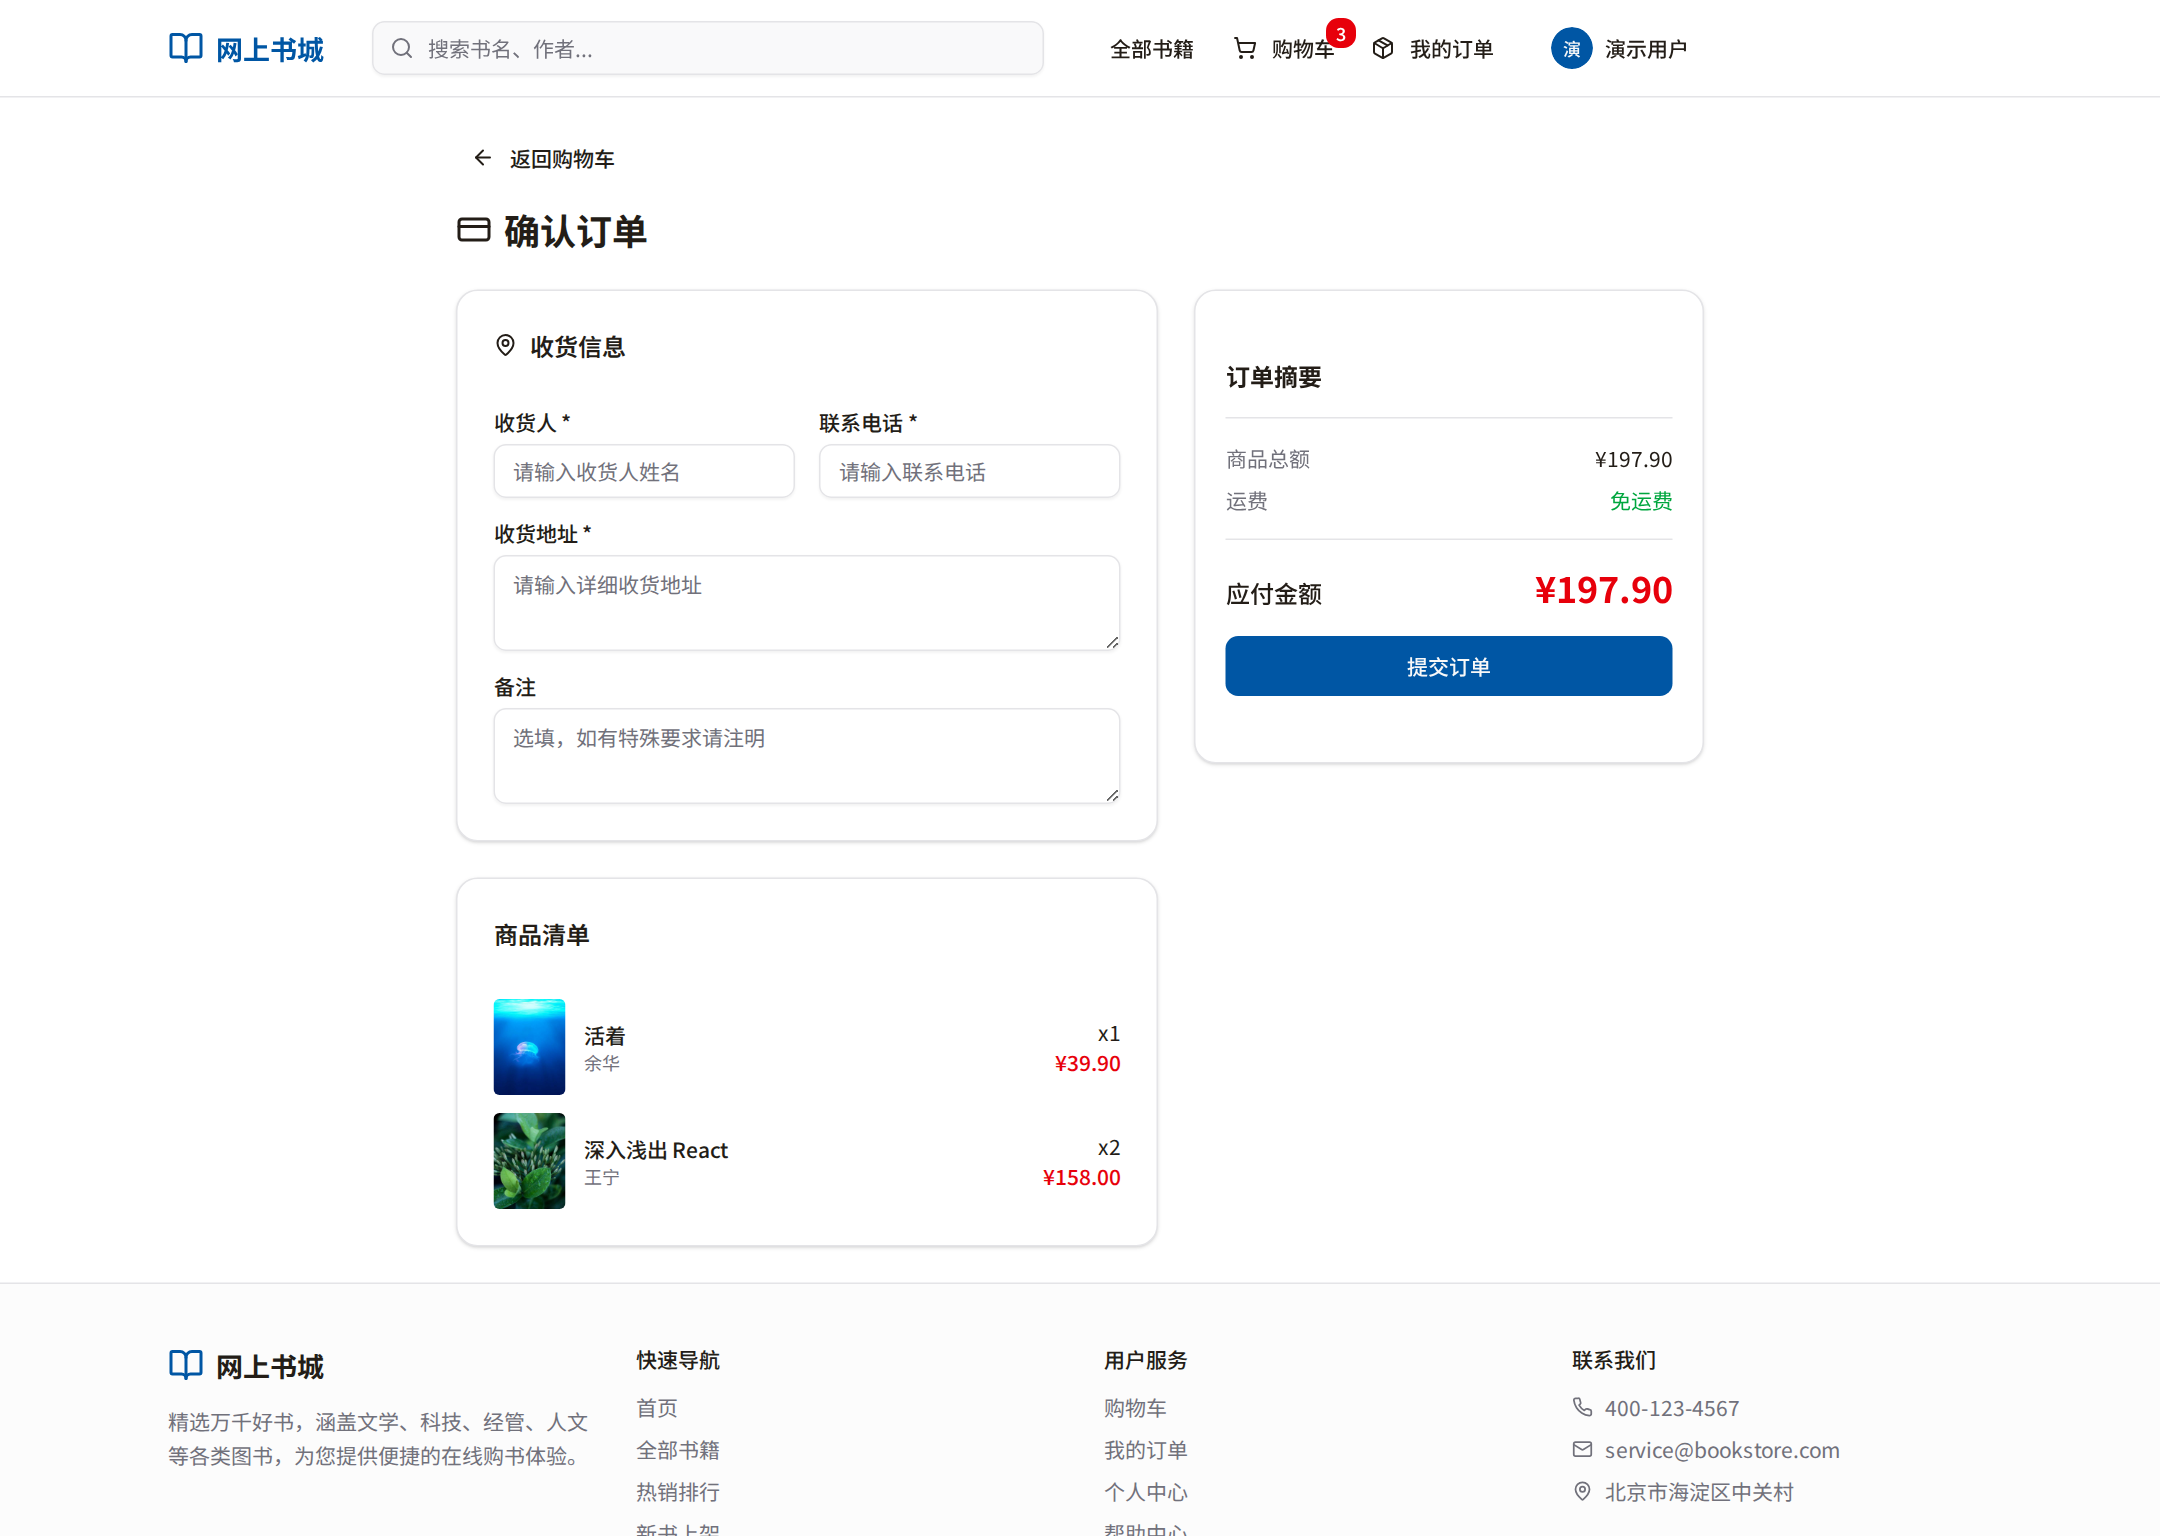
\includegraphics[width=0.90\textwidth]{screenshots/05-user-checkout.png}
  \caption{订单结算界面}
  \label{fig:checkout}
\end{figure}

\subsubsection{订单查询、订单详情与个人中心}

订单列表页以时间倒序展示历史订单，每条记录显示订单编号、下单时间、商品数量、总金额与当前状态。对于待支付订单，用户可继续执行模拟支付；点击记录后可进入订单详情页，查看收货信息、订单明细与状态流转结果。个人中心允许用户修改用户名与邮箱，修改后即时反映至顶部导航栏。

\begin{figure}[H]
  \centering
  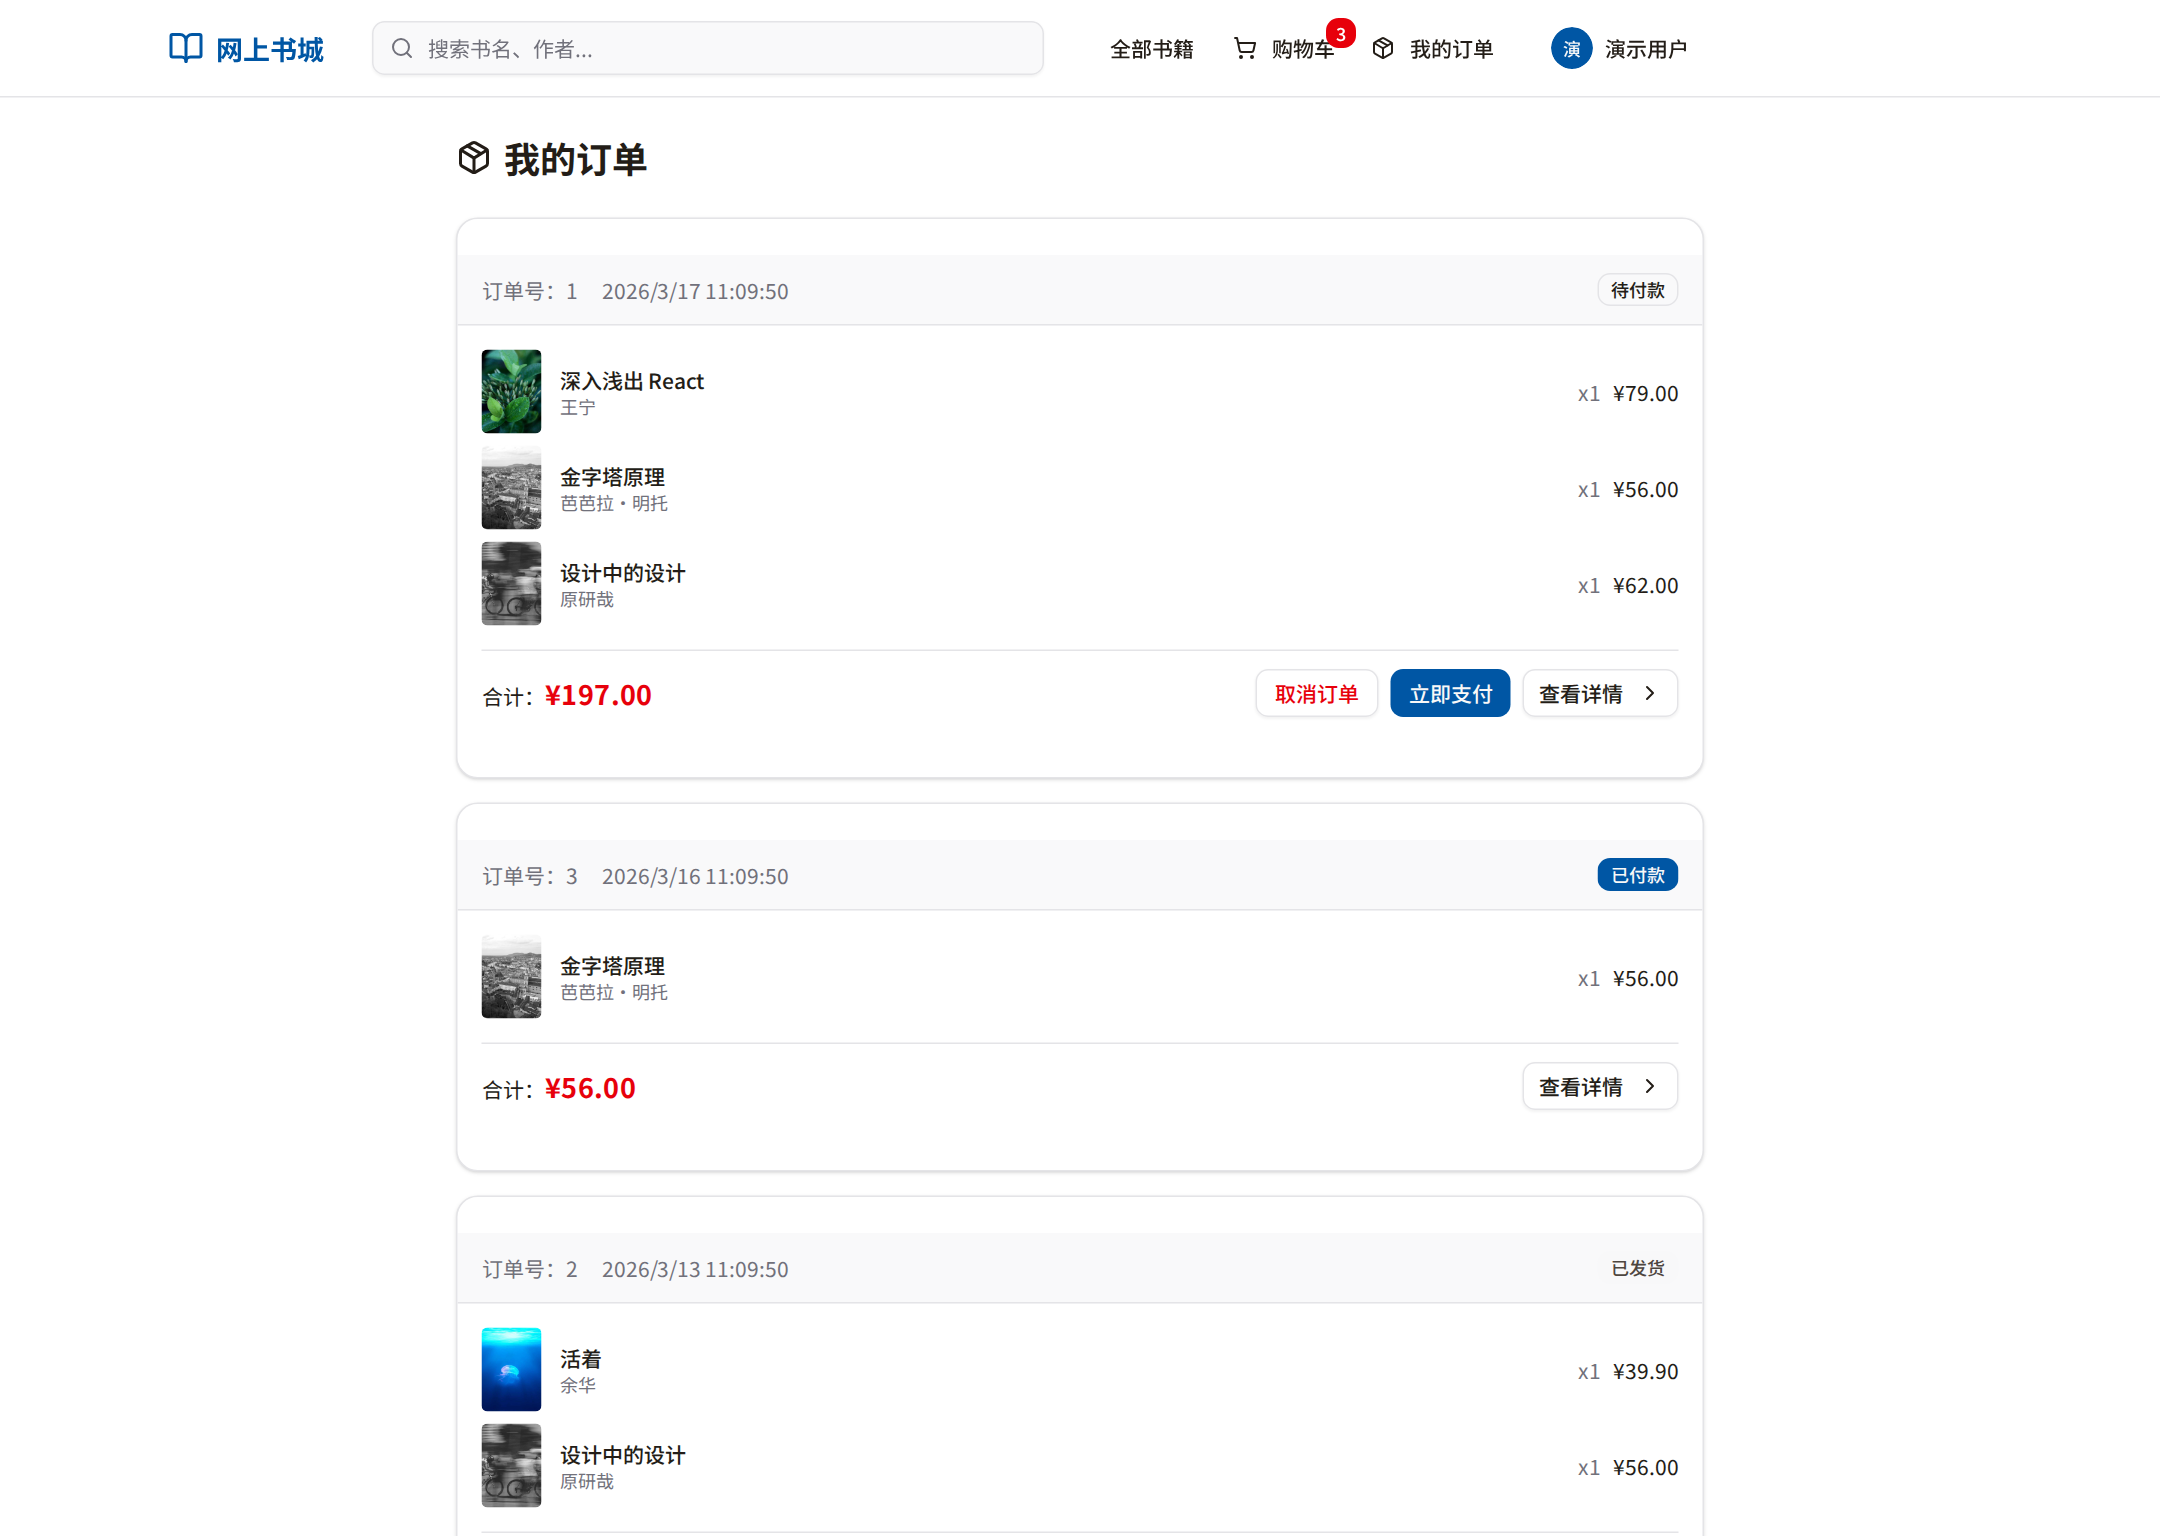
\includegraphics[width=0.90\textwidth]{screenshots/06-user-orders.png}
  \caption{用户订单列表界面}
  \label{fig:orders}
\end{figure}

\begin{figure}[H]
  \centering
  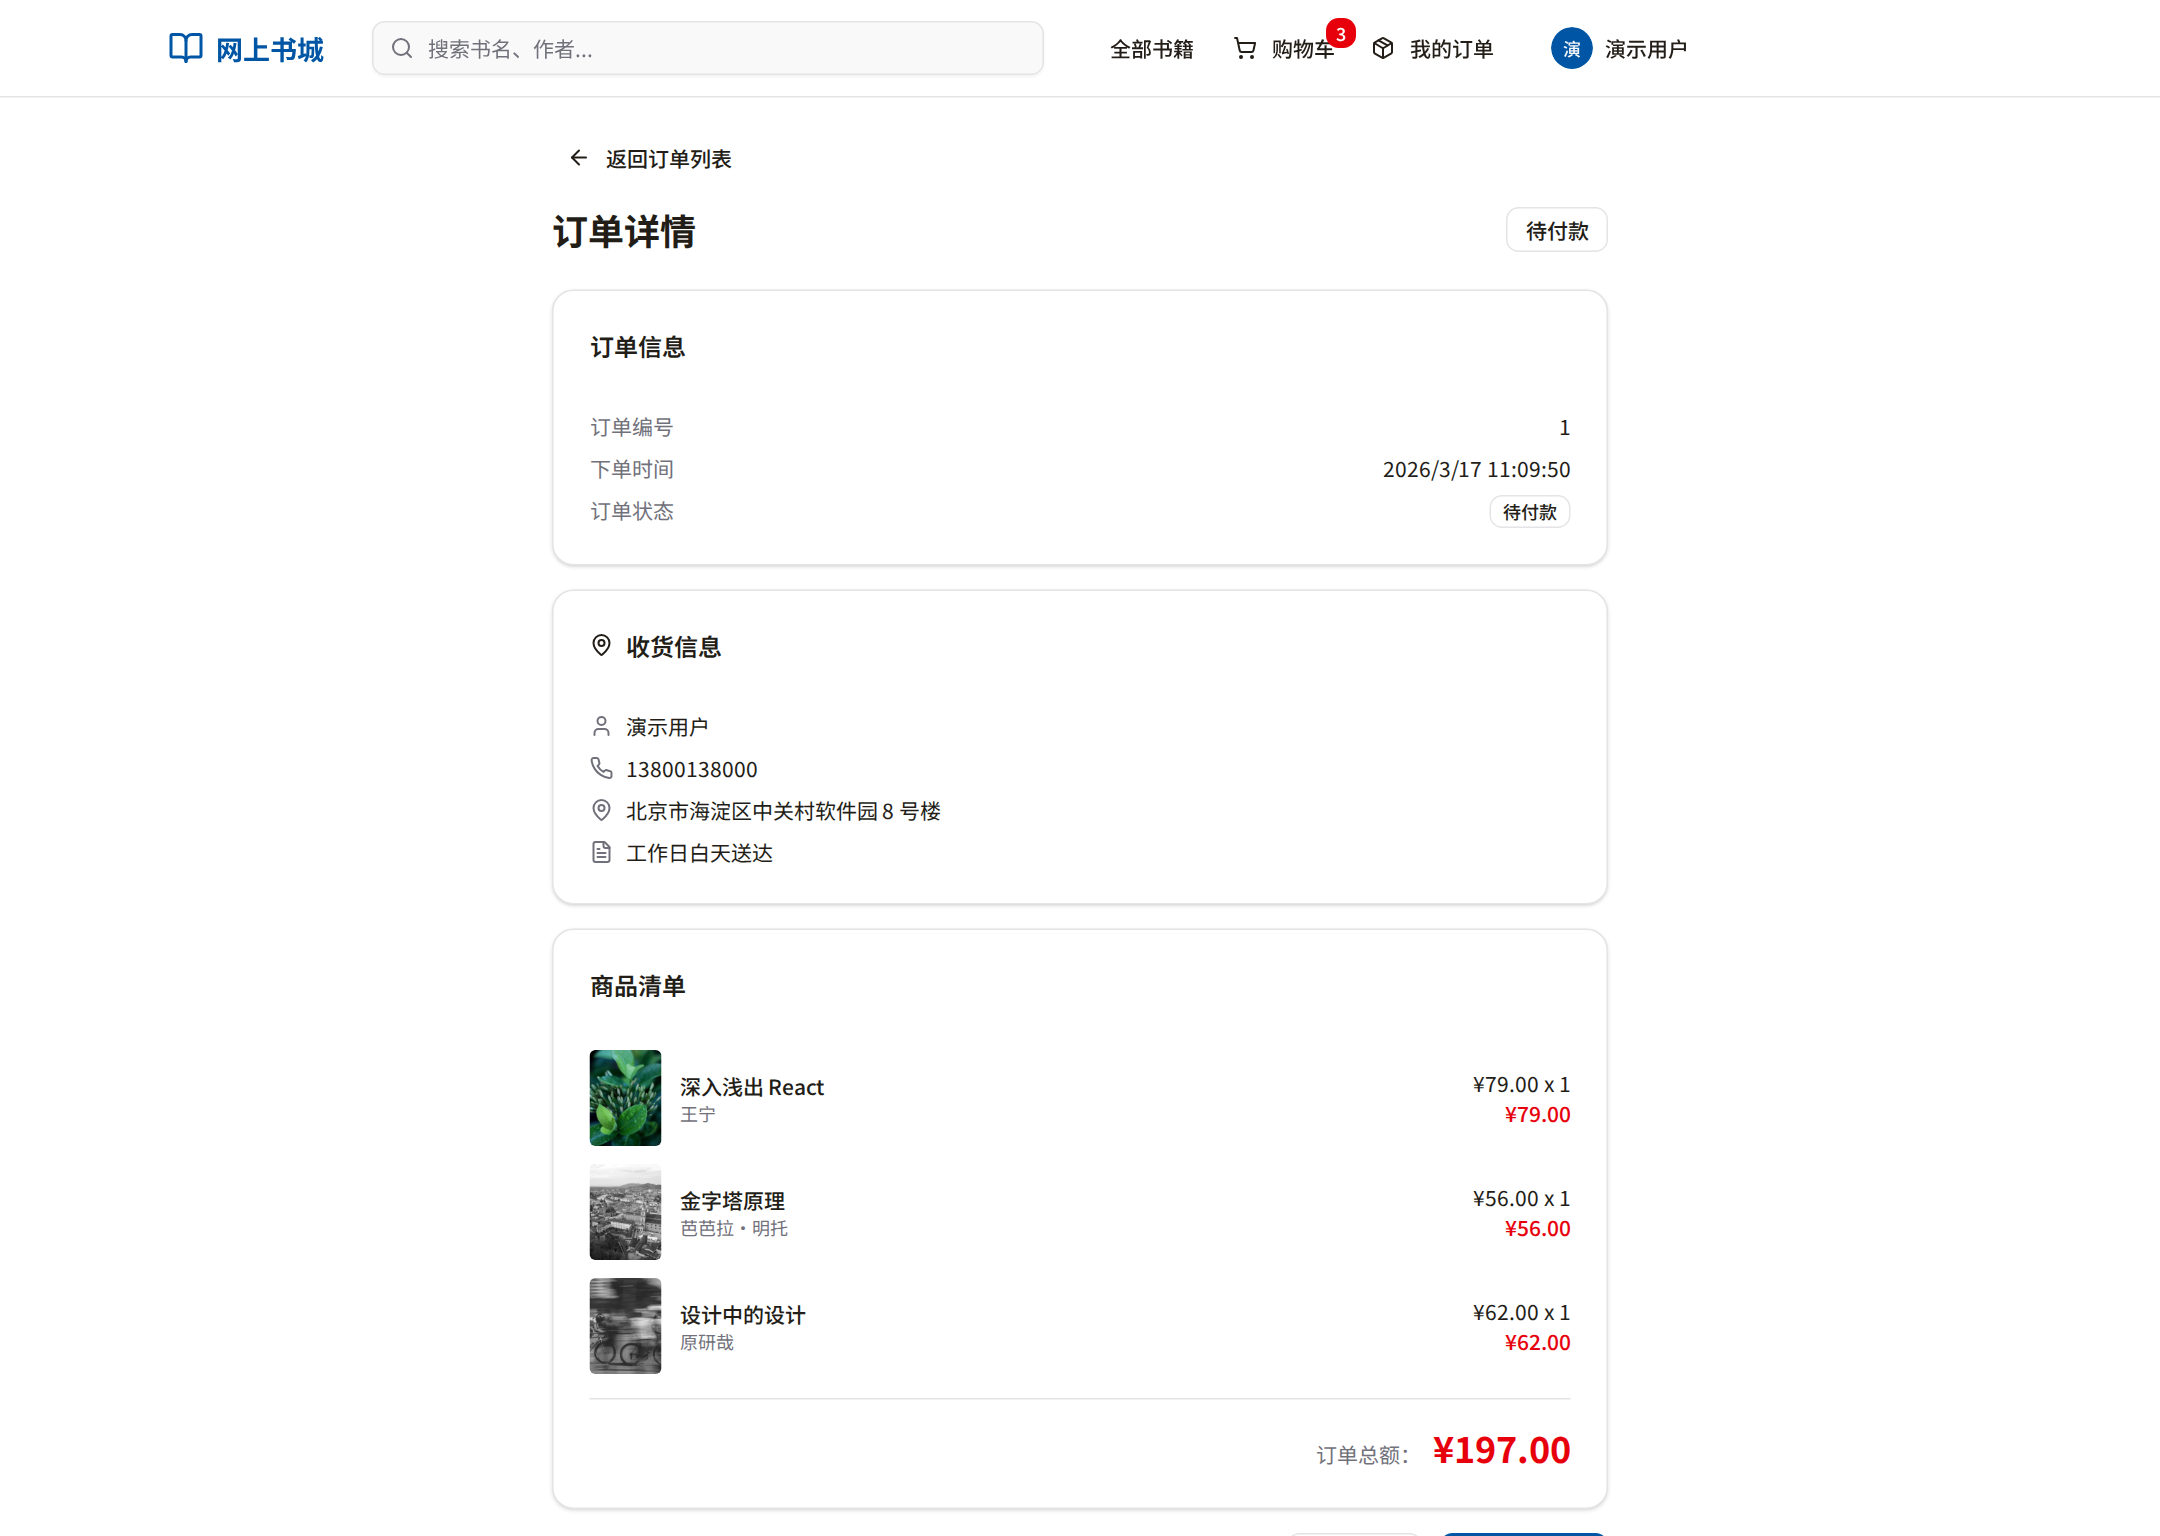
\includegraphics[width=0.90\textwidth]{screenshots/07-user-order-detail.png}
  \caption{用户订单详情界面}
  \label{fig:order-detail}
\end{figure}

\begin{figure}[H]
  \centering
  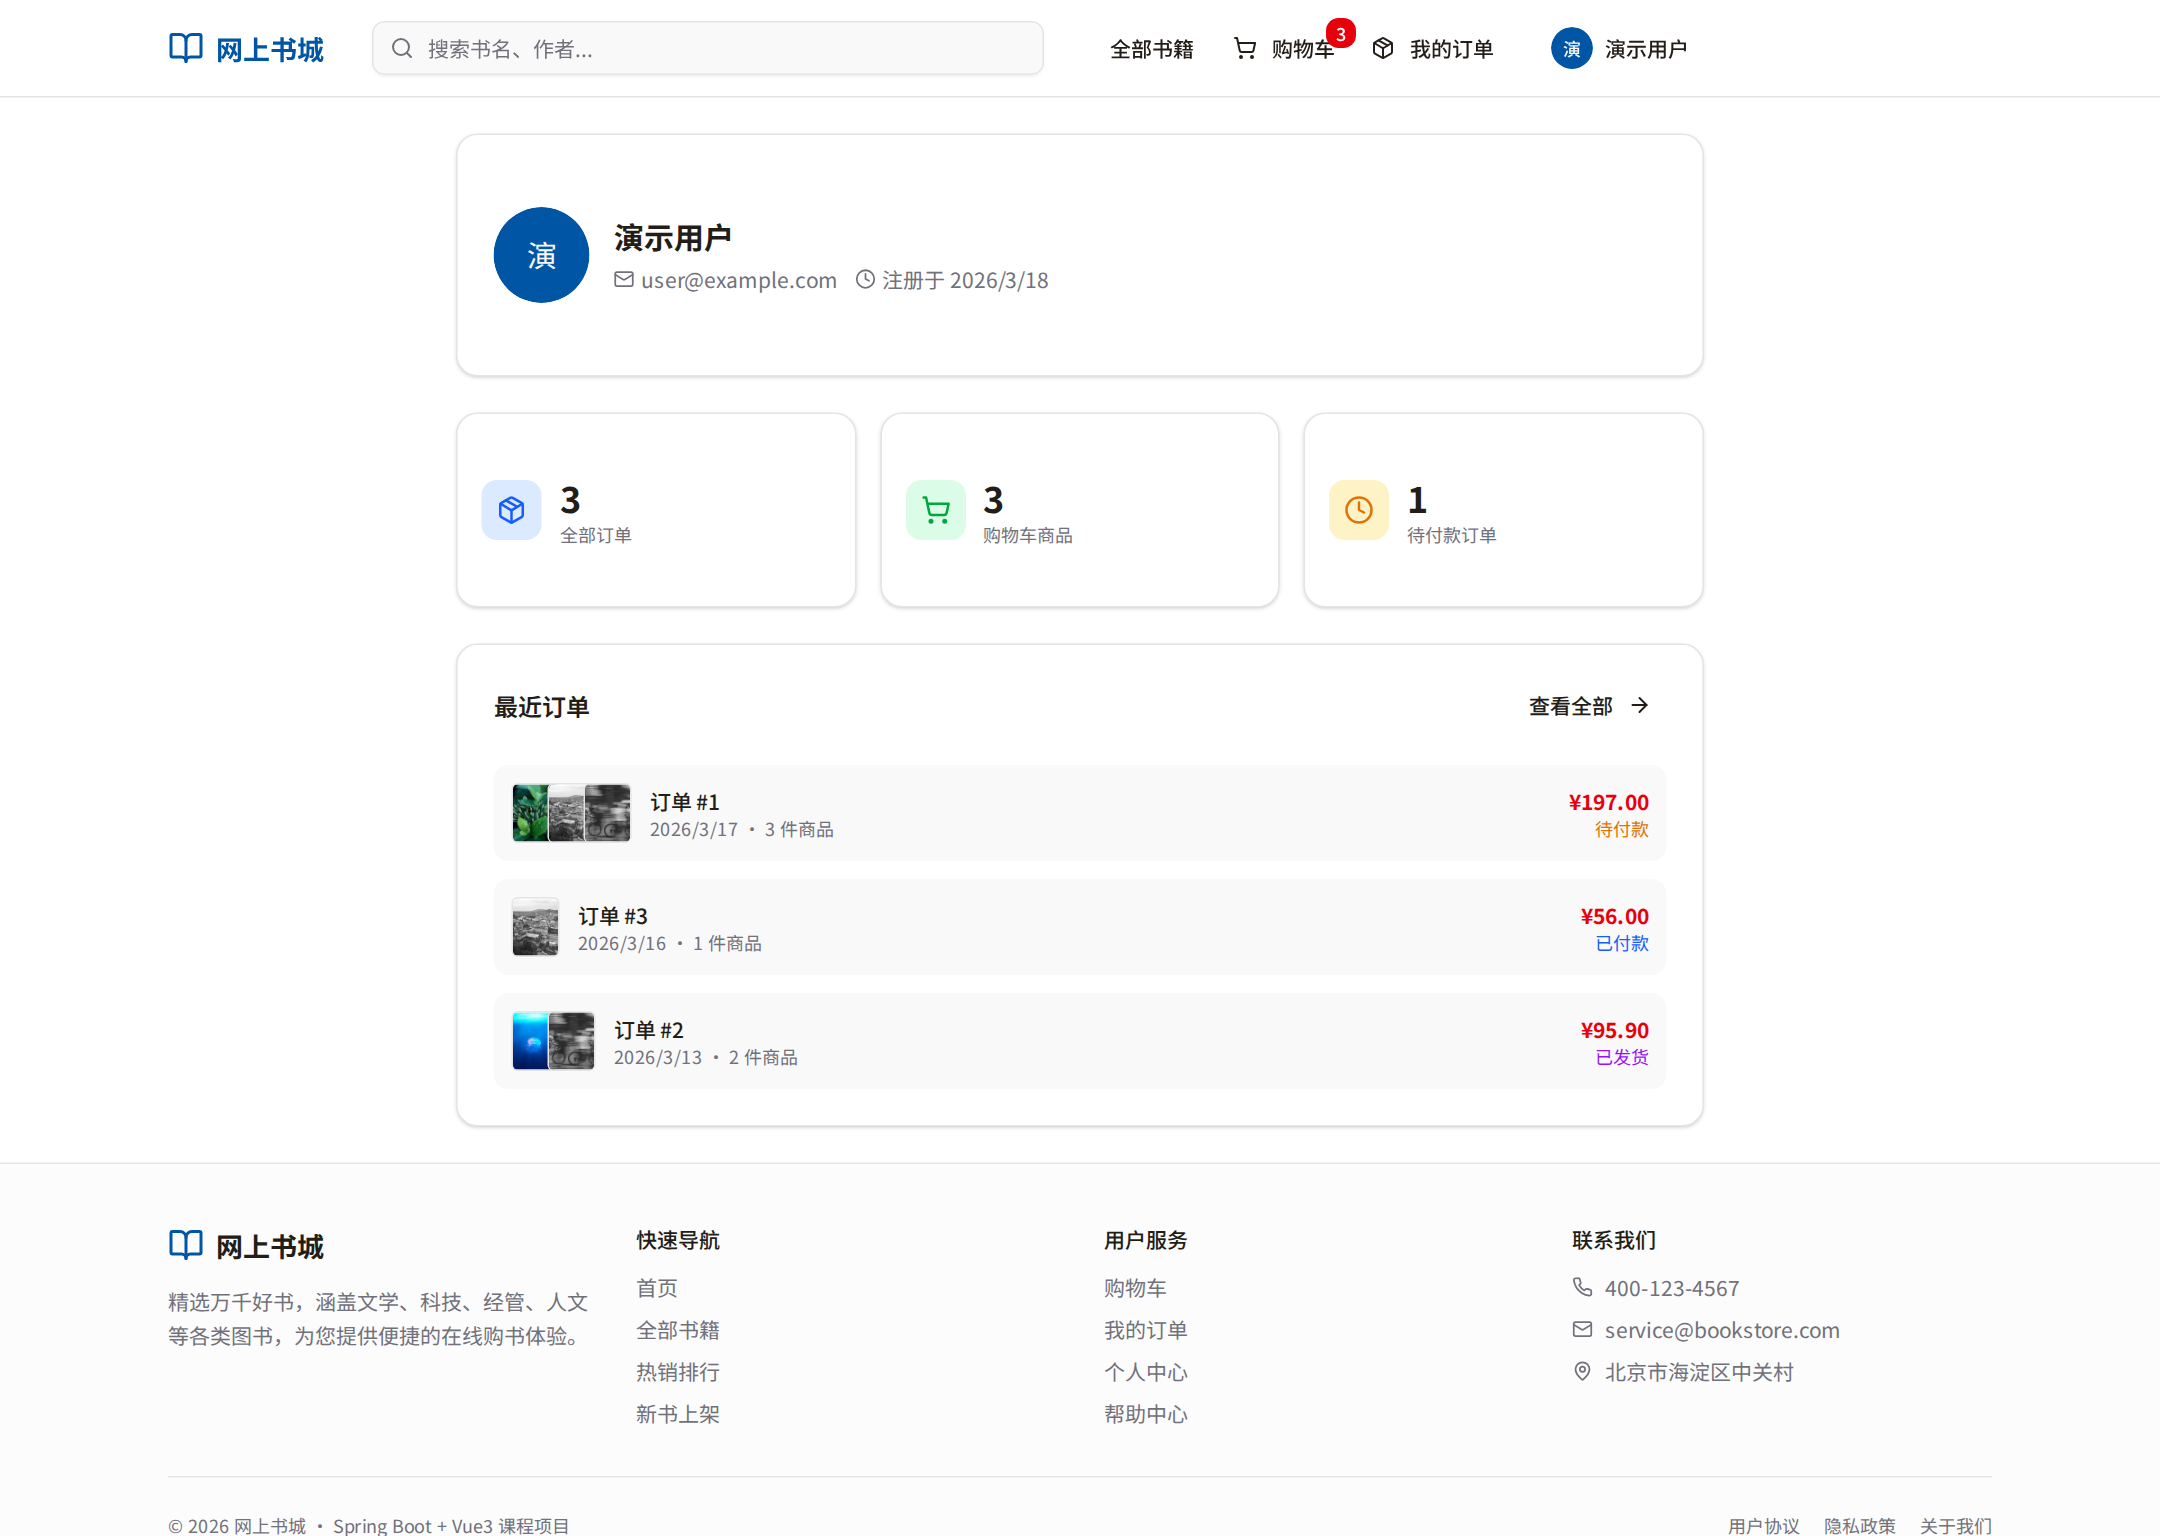
\includegraphics[width=0.90\textwidth]{screenshots/08-user-profile.png}
  \caption{个人中心界面}
  \label{fig:profile}
\end{figure}

\subsection{管理员端界面实现}

\subsubsection{管理后台首页}

管理后台首页以数据看板形式展示总订单数、总销售额、图书总数与注册用户数四项核心指标，各项通过独立tRPC查询获取并以卡片形式并排展示，管理员可一眼掌握系统整体运营状态。

\begin{figure}[H]
  \centering
  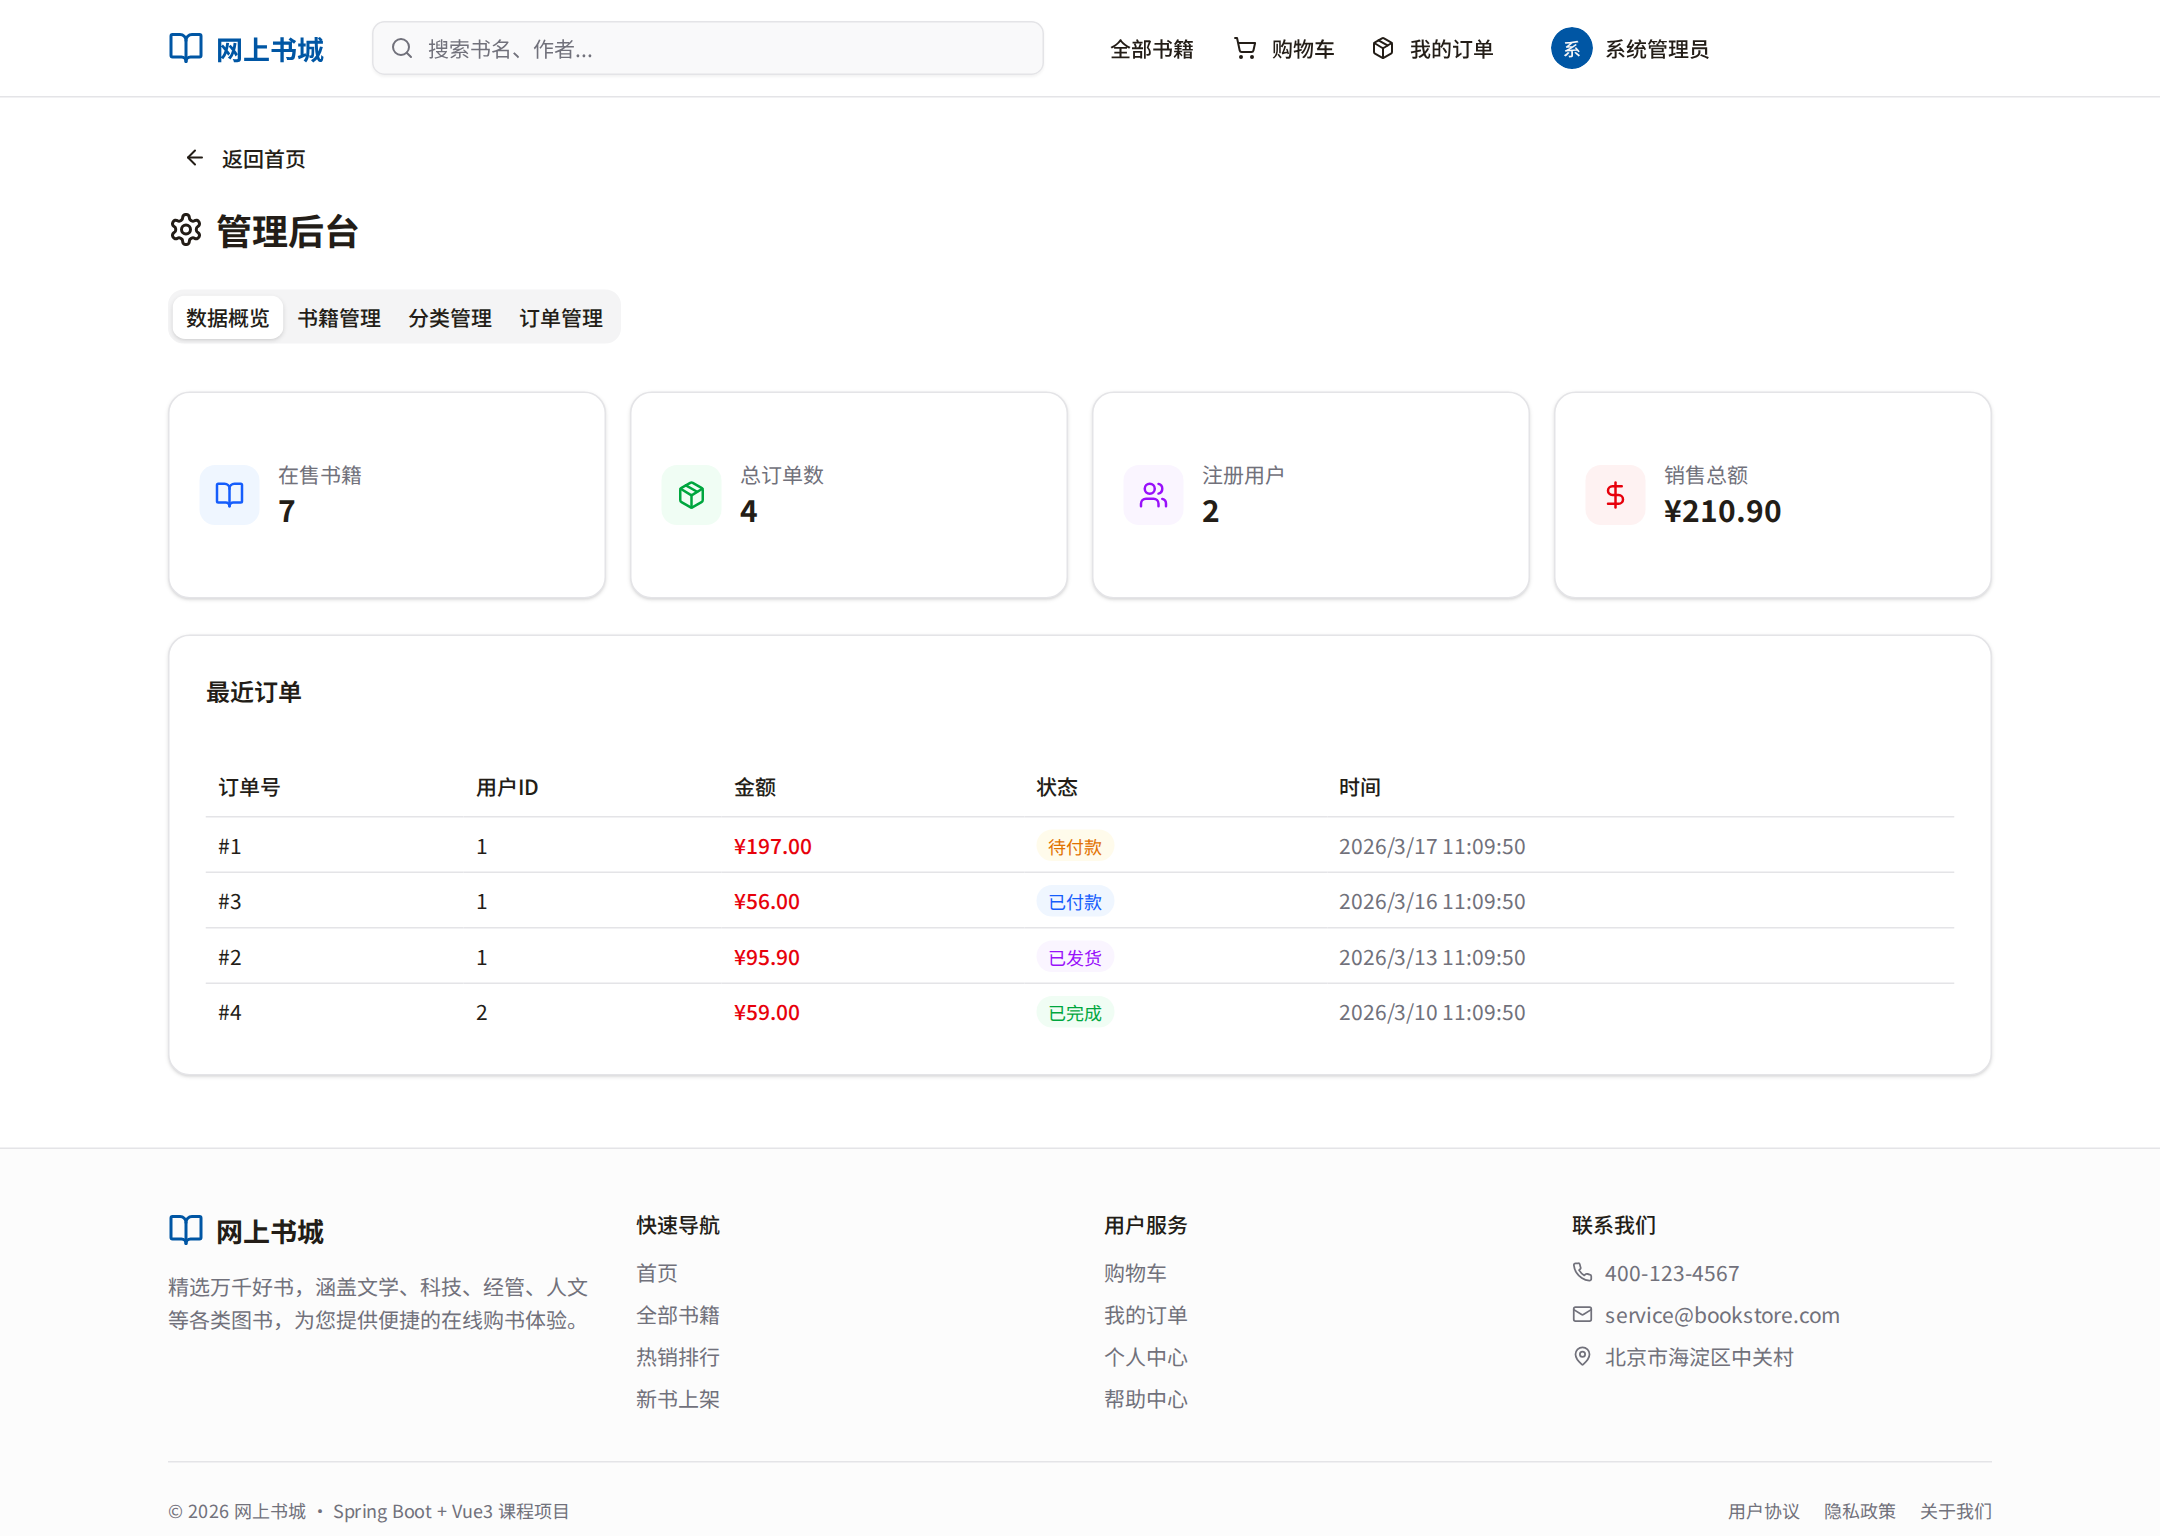
\includegraphics[width=0.90\textwidth]{screenshots/09-admin-dashboard.png}
  \caption{管理后台首页}
  \label{fig:admin-dashboard}
\end{figure}

\subsubsection{书籍与分类管理}

书籍管理提供完整增删改查能力，新增与编辑通过弹窗表单完成，表单字段与服务端Zod Schema保持类型一致；管理员除可查看在售图书外，还可查看已下架图书并执行恢复上架操作。分类管理支持新增、编辑与删除，删除分类时系统会同步解除相关图书的分类关联，避免产生悬空引用数据。

\begin{figure}[H]
  \centering
  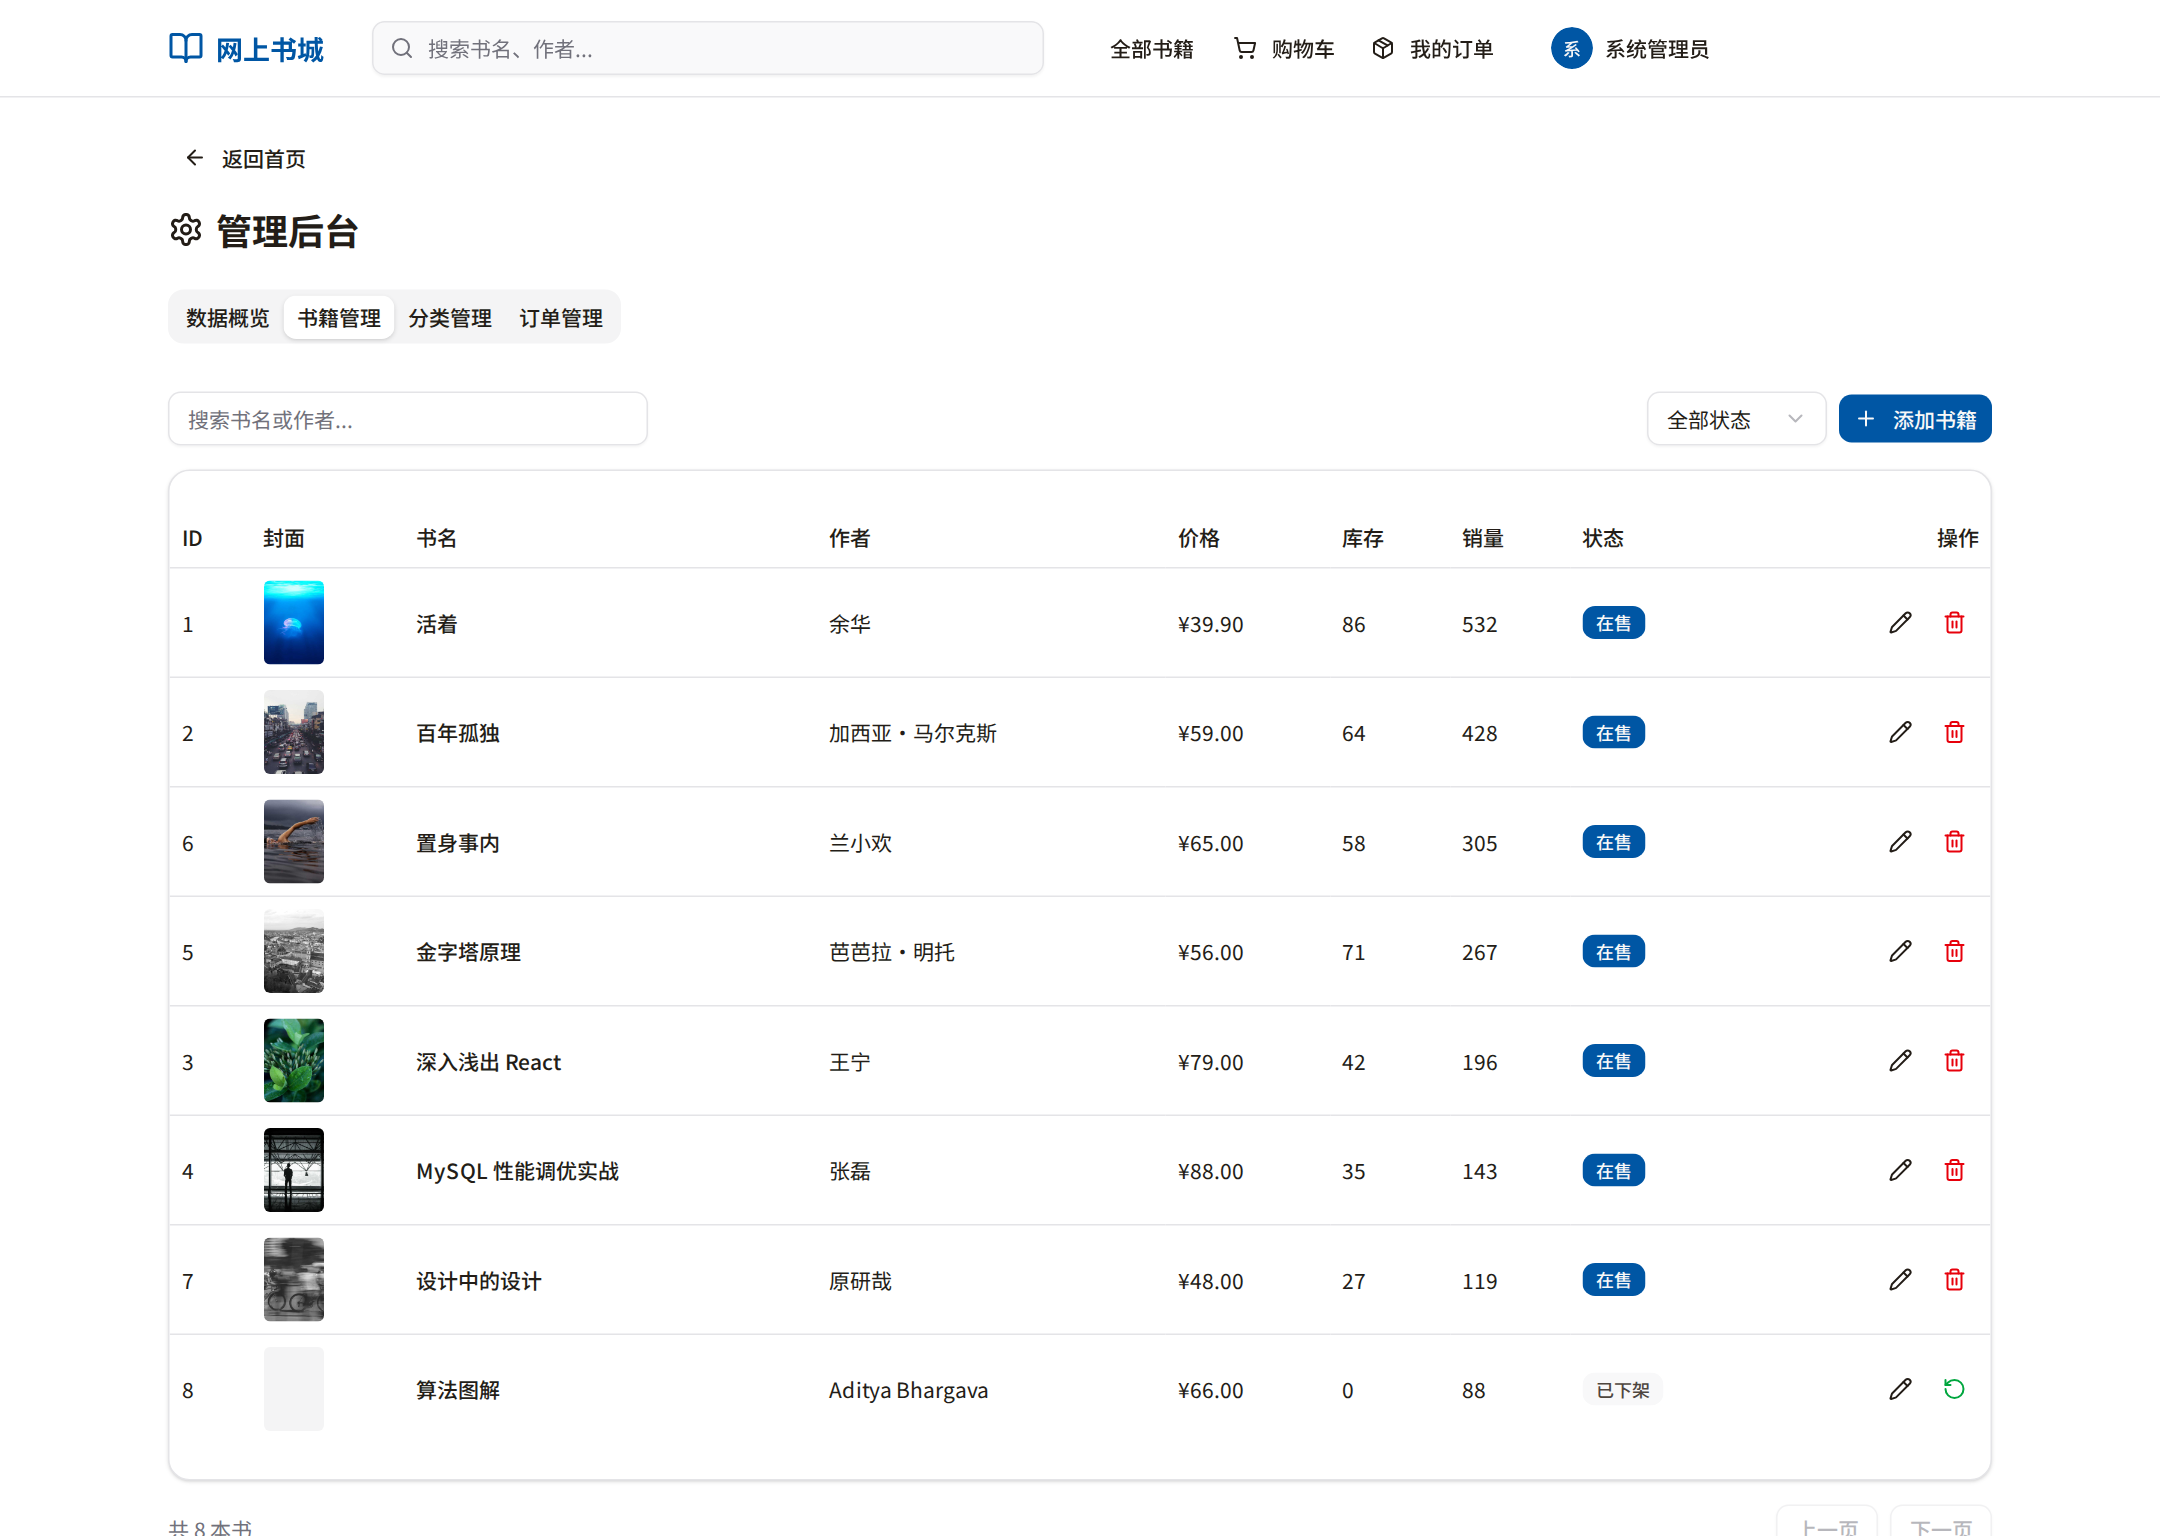
\includegraphics[width=0.90\textwidth]{screenshots/10-admin-books.png}
  \caption{书籍管理界面}
  \label{fig:admin-books}
\end{figure}

\begin{figure}[H]
  \centering
  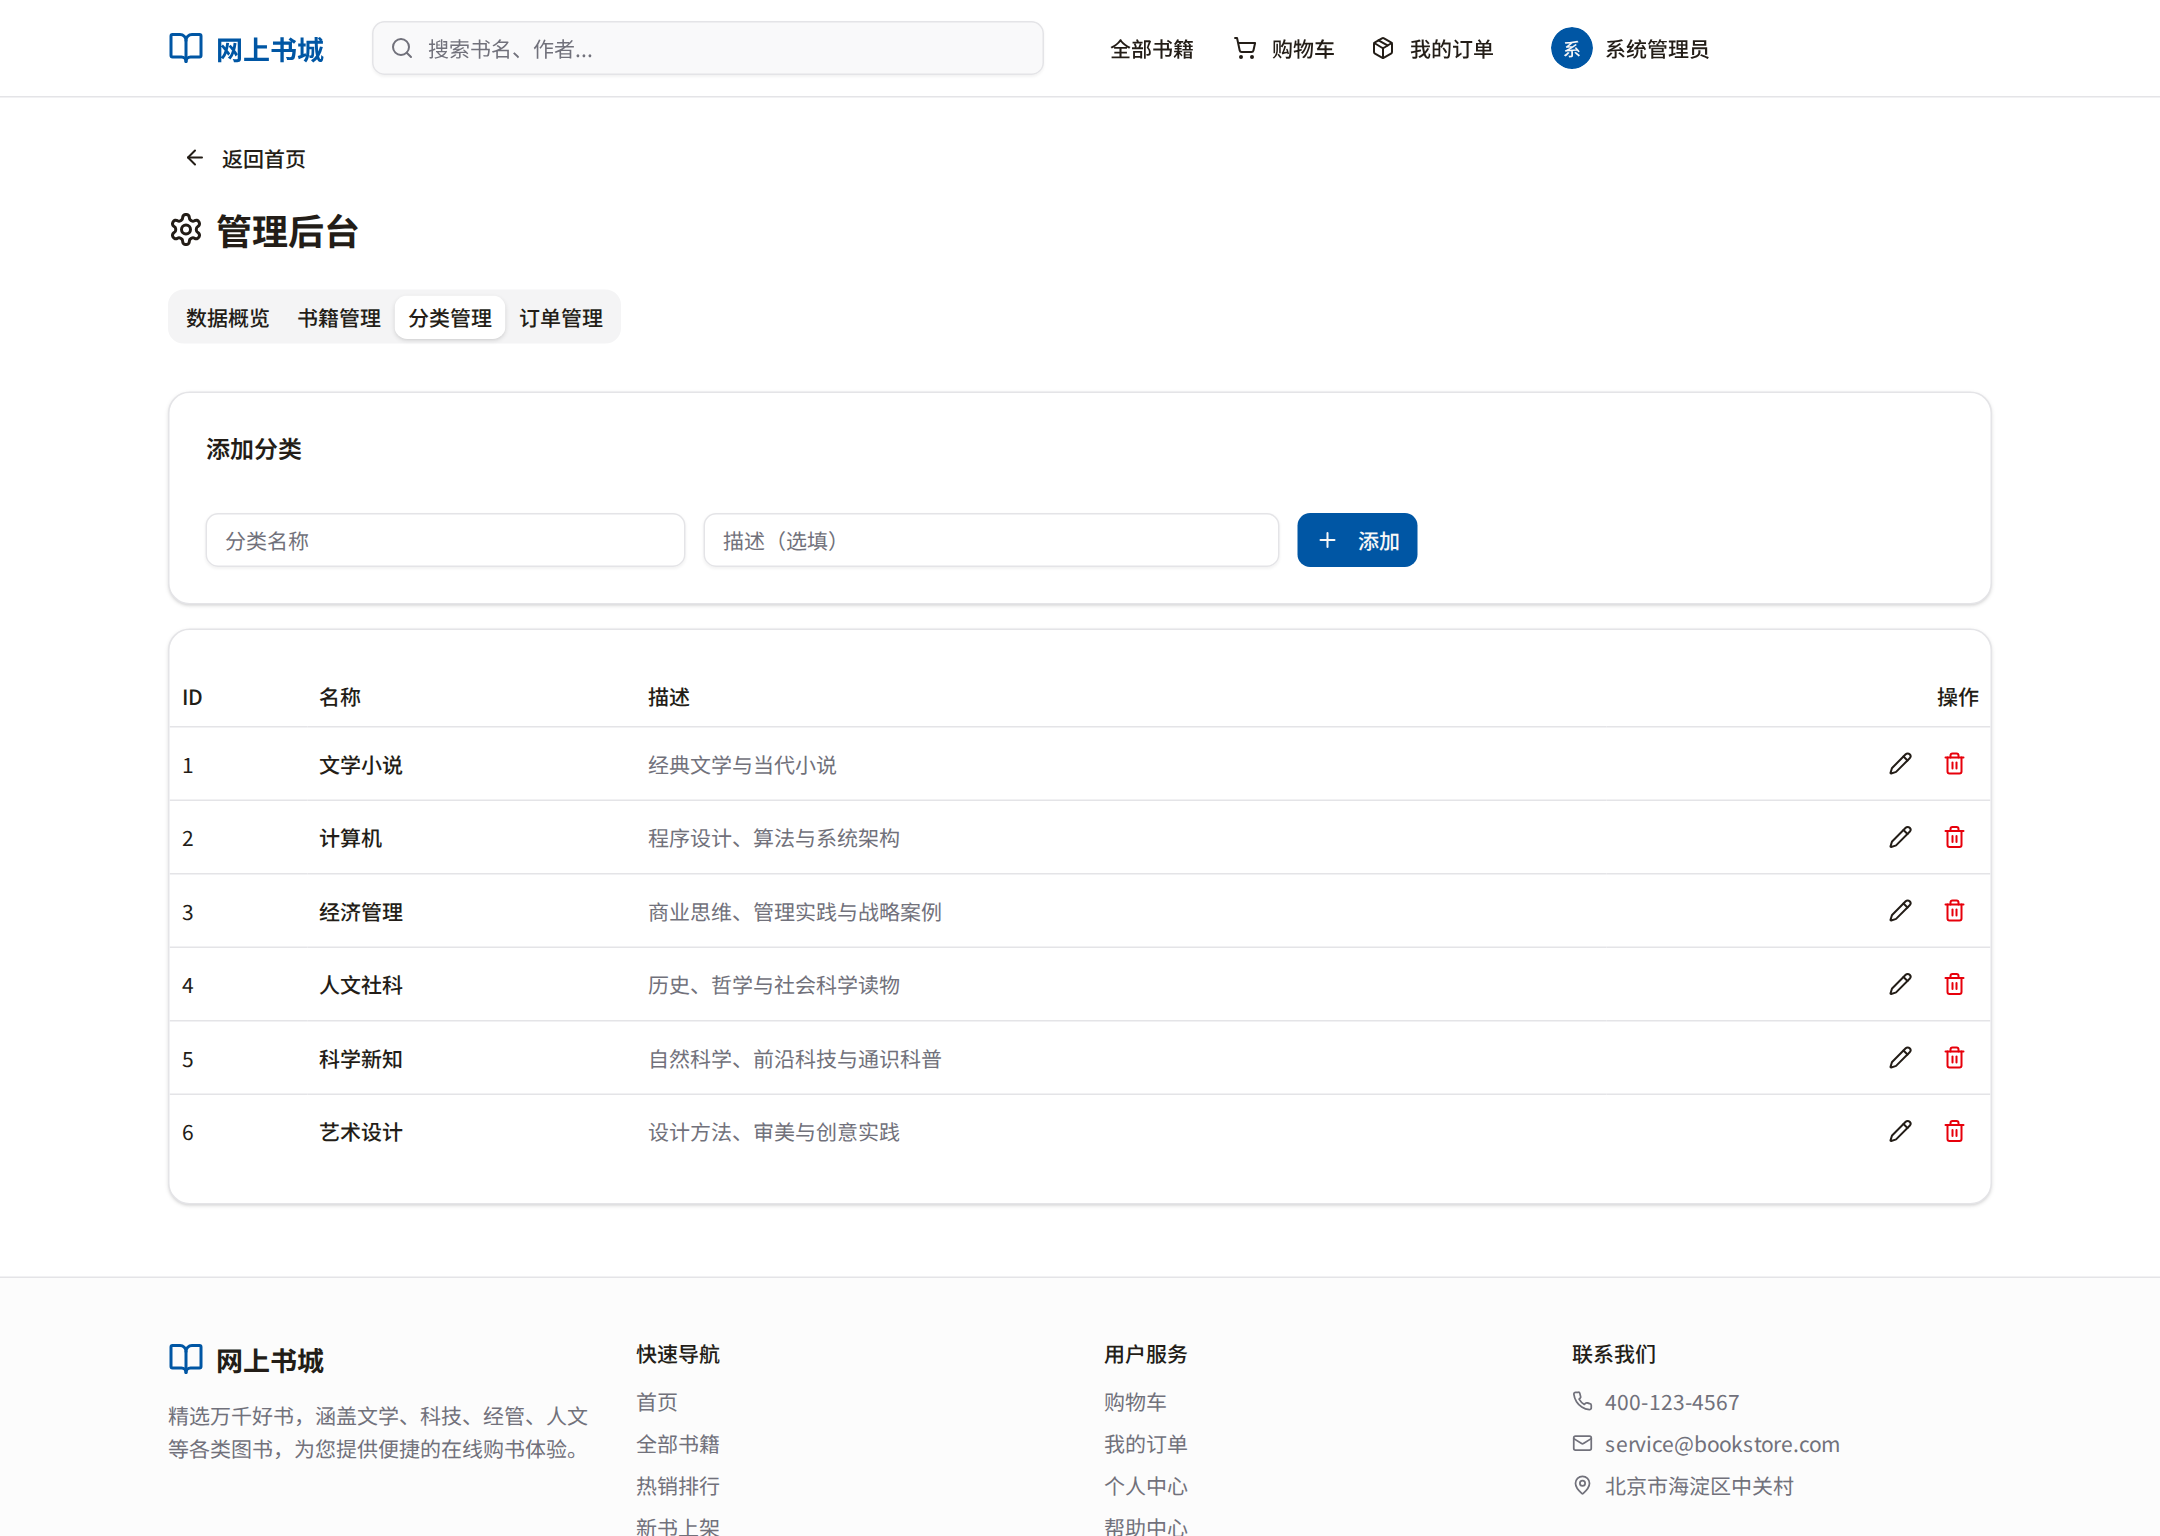
\includegraphics[width=0.90\textwidth]{screenshots/11-admin-categories.png}
  \caption{分类管理界面}
  \label{fig:admin-categories}
\end{figure}

\subsubsection{订单管理}

订单管理页以分页表格展示全部订单，支持按状态筛选。状态流转单向不可逆，由服务端接口强制校验，防止误操作回退订单状态。

\begin{figure}[H]
  \centering
  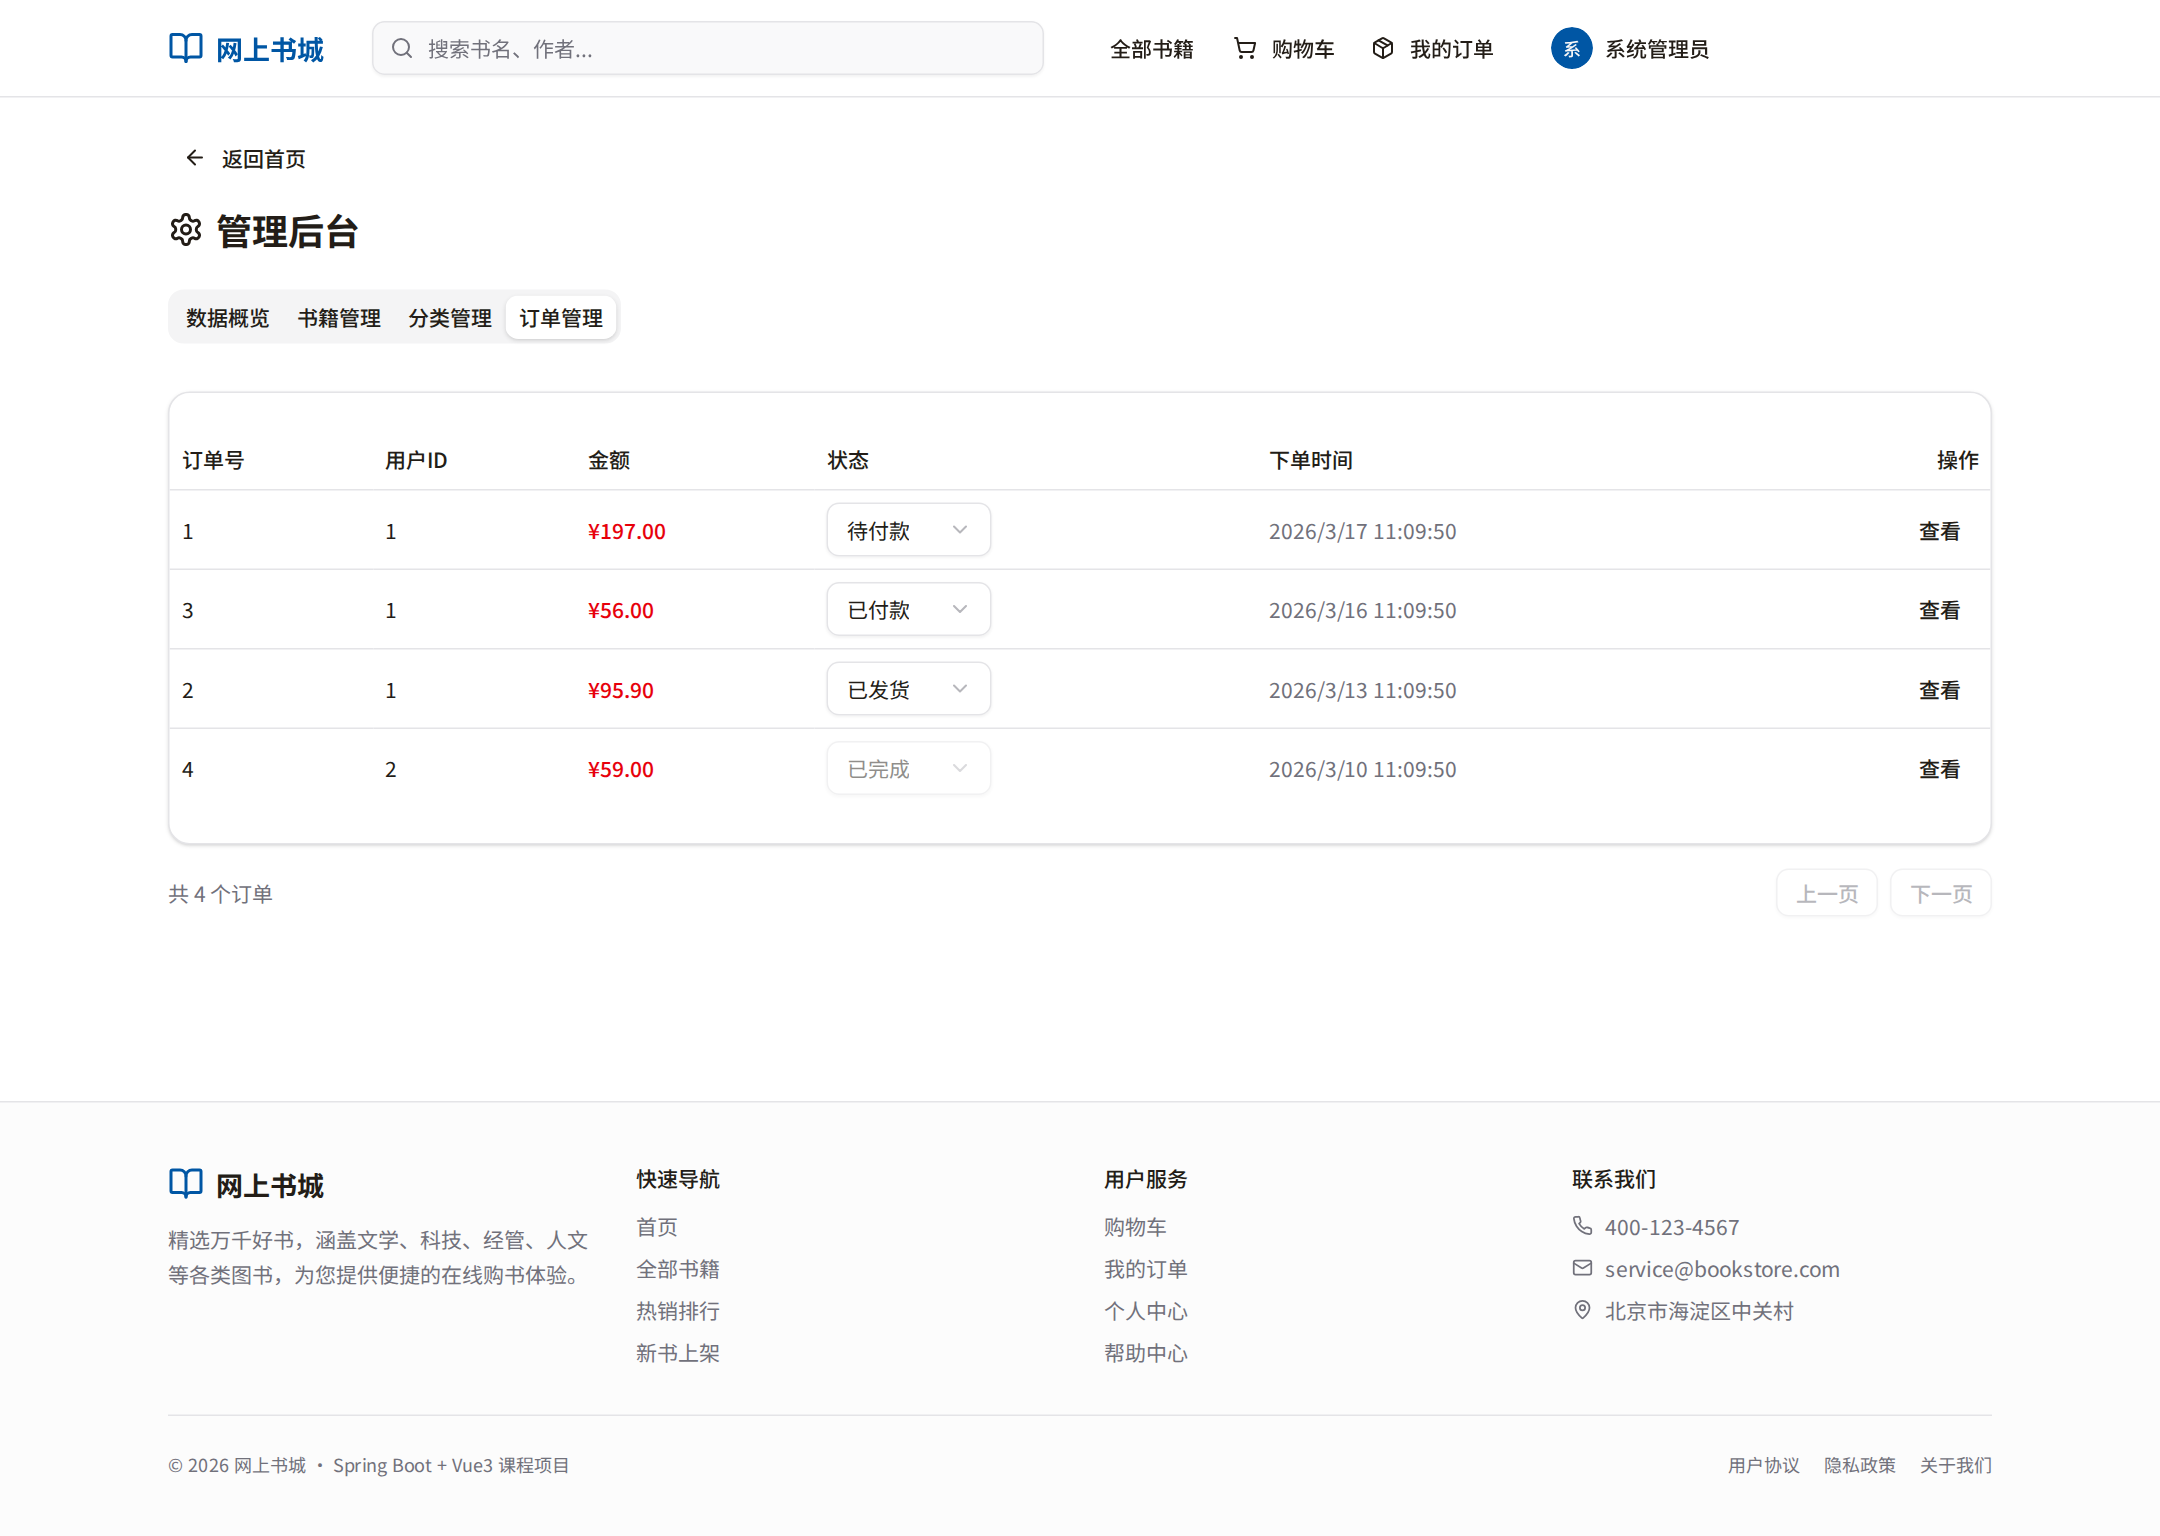
\includegraphics[width=0.90\textwidth]{screenshots/12-admin-orders.png}
  \caption{订单管理界面}
  \label{fig:admin-orders}
\end{figure}

\subsection{关键技术实现}

\subsubsection{tRPC端到端类型安全}

以书籍列表接口为例，服务端通过Zod定义输入Schema，Drizzle ORM查询结果类型由TypeScript自动推导，前端调用时无需手写任何类型注解，编译器即可检查字段名称与类型是否匹配。这一链路消除了因接口文档滞后或字段拼写错误导致的运行时故障，将类型错误的暴露时机从运行时提前至编译阶段。

\subsubsection{事务一致性保障}

订单提交流程涉及库存核减与订单记录创建两个写操作，系统通过Drizzle ORM的事务API将二者包裹在同一数据库事务中。若库存不足或任一写操作失败，事务自动回滚，购物车数据保持不变，不会出现已扣库存但无订单记录的数据不一致状态。

\subsection{本章小结}

本章从用户端界面、管理员端界面与关键技术实现三个层面对系统实现过程进行了说明。可以看出，前端页面展示与后端业务规则之间并非简单拼接关系，而是通过共享类型、统一校验与事务机制共同保证了系统交互体验与业务一致性。


% ======== 第5章 测试与验证 ========
\section{测试与验证}

\subsection{测试环境}

系统测试在本地开发环境下进行，硬件配置为x86-64架构CPU、16\ GB内存；软件环境为Node.js 20、MySQL 8.0、pnpm 10。前端通过Vite开发服务器运行，后端以\texttt{tsx watch}模式启动，数据库使用预置演示数据。

\subsection{功能测试}

功能测试按照第2章需求规格逐项验证，测试用例覆盖用户端与管理员端全部核心业务流程，结果如表\ref{tab:func-test}所示。

\begin{table}[H]
  \centering
  \caption{功能测试结果汇总}
  \label{tab:func-test}
  \small
  \begin{tabularx}{\textwidth}{p{3.1cm} p{7.0cm} p{1.8cm}}
    \toprule
    测试模块 & 测试用例 & 测试结果 \\
    \midrule
    用户会话与权限 & 登录后访问受保护页面、未登录跳转、普通用户访问后台拒绝 & 通过 \\
    图书浏览 & 首页展示、关键词搜索、分类筛选、排序切换 & 通过 \\
    图书详情 & 详情展示、库存显示、数量校验 & 通过 \\
    购物车 & 加购、数量增减、删除、金额汇总 & 通过 \\
    订单结算 & 表单校验、库存核减、订单生成、事务回滚 & 通过 \\
    订单查询 & 列表展示、详情查看、状态显示 & 通过 \\
    个人中心 & 信息展示、修改用户名/邮箱 & 通过 \\
    后台书籍管理 & 新增、编辑、删除、分页展示 & 通过 \\
    后台分类管理 & 新增、编辑、删除（含关联处理）& 通过 \\
    后台订单管理 & 订单列表、状态流转、越权拒绝 & 通过 \\
    \bottomrule
  \end{tabularx}
\end{table}

\subsection{工程化验证}

除面向业务流程的功能测试外，本文还对当前工程产物执行了类型检查、自动化测试、生产构建与关键界面导出验证，结果如表\ref{tab:engineering-checks}所示。这些验证结果说明，系统不仅在页面层面能够完成演示，也具备较好的工程稳定性与可交付性。

\begin{table}[H]
  \centering
  \caption{工程化验证结果}
  \label{tab:engineering-checks}
  \small
  \begin{tabularx}{\textwidth}{p{2.8cm} p{3.8cm} X}
    \toprule
    验证项目 & 执行方式 & 结果说明 \\
    \midrule
    类型检查 & \texttt{pnpm check} & 执行通过，说明前后端共享类型定义在当前版本下无编译错误。 \\
    自动化测试 & \texttt{pnpm test} & 共运行2个测试文件、27项测试，全部通过，覆盖鉴权登出与书城核心业务逻辑。 \\
    生产构建验证 & \texttt{pnpm build} & 前后端构建均通过，成功生成生产产物；构建日志提示前端主JS包体仍偏大，后续可继续进行路由级代码分割优化。 \\
    界面导出验证 & \shortstack[l]{\texttt{node}\\\texttt{capture\_screenshots.mjs}} & 在\texttt{thesis\_assets}目录执行后，成功导出用户端与管理员端关键界面截图，可用于答辩演示和论文插图。 \\
    \bottomrule
  \end{tabularx}
\end{table}

从工程验证结果可以看出，当前系统已经具备较好的基础质量保障能力。其中，类型检查与自动化测试确保了接口契约与主要业务逻辑的稳定性，生产构建成功则说明项目能够以发布形态打包部署。需要指出的是，构建过程中仍出现较大的前端主包体积提示，这为后续的性能优化提供了明确方向。

\subsection{安全性测试}

针对系统主要安全约束进行验证：直接访问管理员接口（\texttt{adminProcedure}）时，服务端返回未授权错误，前端同步跳转至登录页；以普通用户Token调用管理员接口时，服务端校验角色后拒绝请求；Cookie中的JWT篡改后，服务端签名验证失败并清除会话。上述测试结果表明系统安全边界实现符合预期，权限控制不依赖前端路由守卫作为唯一防线。

\subsection{类型安全验证}

在开发阶段人工引入若干类型错误（如将接口返回的\texttt{price}字段当作\texttt{number}使用，而实际Schema定义为\texttt{string}），TypeScript编译器在保存文件后即刻在前端调用处标红，IDE内联提示明确指向服务端Schema定义位置。这一验证表明，tRPC的端到端类型推导在实际工程场景中能够有效拦截接口契约不一致问题。

\subsection{本章小结}

本章从测试环境、功能测试、工程化验证、安全性验证和类型安全验证五个方面对系统进行了综合验证。结果表明，网上书城系统已能够稳定完成论文要求的核心业务流程，同时在类型安全、权限控制和工程构建层面具备较好的可验证性与可演示性。


% ======== 第6章 总结与展望 ========
\section{总结与展望}

\subsection{工作总结}

本文围绕网上书城系统的设计与实现展开研究，以端到端类型安全为核心工程理念，选用React、tRPC与Drizzle ORM构建前后端分离的全栈TypeScript应用。系统完整实现了用户端的图书浏览、检索、购物车、订单提交与跟踪等购书全流程，以及管理员端的书籍管理、分类管理、订单管理与数据看板等后台能力。

在工程实践层面，本文的主要贡献体现在以下三个方面。其一，验证了tRPC在中小型电商场景的可行性。通过将服务端Router的TypeScript类型直接传递至前端，接口契约的一致性由编译器保证，消除了传统REST开发中因接口文档滞后引发的联调摩擦。其二，实践了Drizzle ORM的Schema优先设计范式。以单一TypeScript文件作为数据库结构与类型定义的唯一来源，数据迁移与类型推导统一维护，减少了多处同步的维护负担。其三，在订单提交等关键写操作上通过数据库事务保证了业务一致性，系统在测试阶段未出现库存与订单记录不一致的情况。

\subsection{不足与展望}

受开发周期与个人能力所限，当前系统在以下几个方面仍有较大的改进空间。

\textbf{支付集成。}现有系统的订单提交流程跳过了真实的支付环节，仅模拟了订单状态的生成。后续可接入微信支付或支付宝的沙箱环境，补全支付回调、退款等完整支付链路。

\textbf{搜索能力。}当前关键词搜索基于MySQL的\texttt{LIKE}查询实现，在数据量增大后存在性能瓶颈，且不支持分词与相关性排序。引入Elasticsearch或MySQL全文索引可显著提升检索体验。

\textbf{图片存储。}书籍封面图片目前以外部URL字符串形式存储，依赖第三方图床的可用性。后续可对接云存储服务（如AWS S3或阿里云OSS），通过预签名URL实现安全的图片上传与访问。

\textbf{性能优化。}当前系统未引入服务端缓存层，热门图书列表的数据库查询在高并发场景下存在重复计算问题；同时，生产构建结果显示前端主包体积仍偏大。后续可在接口层引入Redis缓存，并结合路由级代码分割与手动Chunk拆分进一步降低首屏加载压力。

\textbf{测试覆盖率。}当前仅进行了手工功能测试，缺乏自动化单元测试与端到端测试。后续可引入Vitest对tRPC过程函数编写单元测试，使用Playwright对核心购书流程编写端到端测试，以持续集成流水线保证代码质量。

综上，本文在有限的工程实践范围内，初步探索了端到端类型安全架构在电商系统中的应用价值，为后续在更大规模、更复杂业务场景下的深入研究提供了参考基础。

\newpage
\section*{致谢}
\addcontentsline{toc}{section}{致谢}

在本论文的选题、开发与撰写过程中，我得到了许多老师、同学与家人的帮助与支持。在此谨向所有关心和帮助过我的人表示诚挚的感谢。

首先，衷心感谢指导教师在论文选题、研究思路、系统实现与论文修改过程中给予的悉心指导。老师严谨的治学态度和认真负责的工作作风，使我在毕业设计过程中受益匪浅。

其次，感谢学院各位任课教师在大学阶段的培养，使我系统掌握了软件工程、数据库、Web开发等方面的基础知识，为本系统的设计与实现奠定了扎实基础。感谢同学与朋友在系统测试、界面演示和论文修改阶段提供的建议与帮助。

最后，感谢家人在学习与生活中给予的理解、支持与鼓励，使我能够顺利完成本科阶段的学习任务和毕业论文撰写工作。

\newpage
\section*{参考文献}
\addcontentsline{toc}{section}{参考文献}
\begin{enumerate}[label={[\arabic*]}]
  \item Meta Platforms. React Documentation[EB/OL]. 2024. \url{https://react.dev}.
  \item tRPC Team. tRPC Documentation[EB/OL]. 2024. \url{https://trpc.io/docs}.
  \item Drizzle Team. Drizzle ORM Documentation[EB/OL]. 2024. \url{https://orm.drizzle.team}.
  \item TanStack. TanStack Query Documentation[EB/OL]. 2024. \url{https://tanstack.com/query}.
  \item Wieruch R. The Road to React[EB/OL]. 2022. \url{https://www.robinwieruch.de/the-road-to-learn-react/}.
  \item Abramov D, Nabors R. Introducing react.dev[EB/OL]. 2023. \url{https://react.dev/blog/2023/03/16/introducing-react-dev}.
  \item Fielding R T. Architectural Styles and the Design of Network-based Software Architectures[D/OL]. University of California, Irvine, 2000. \url{https://roy.gbiv.com/pubs/dissertation/top.htm}.
  \item Fowler M. Patterns of Enterprise Application Architecture[M]. Boston: Addison-Wesley, 2002.
  \item OWASP Foundation. OWASP Top 10:2021[EB/OL]. 2021. \url{https://owasp.org/www-project-top-ten/}.
  \item Bierman G, Abadi M, Torgersen M. Understanding TypeScript[C]//ECOOP 2014. Berlin: Springer, 2014: 257--281.
\end{enumerate}

\end{document}
